\documentclass[]{book}
\usepackage{lmodern}
\usepackage{amssymb,amsmath}
\usepackage{ifxetex,ifluatex}
\usepackage{fixltx2e} % provides \textsubscript
\ifnum 0\ifxetex 1\fi\ifluatex 1\fi=0 % if pdftex
  \usepackage[T1]{fontenc}
  \usepackage[utf8]{inputenc}
\else % if luatex or xelatex
  \ifxetex
    \usepackage{mathspec}
  \else
    \usepackage{fontspec}
  \fi
  \defaultfontfeatures{Ligatures=TeX,Scale=MatchLowercase}
\fi
% use upquote if available, for straight quotes in verbatim environments
\IfFileExists{upquote.sty}{\usepackage{upquote}}{}
% use microtype if available
\IfFileExists{microtype.sty}{%
\usepackage{microtype}
\UseMicrotypeSet[protrusion]{basicmath} % disable protrusion for tt fonts
}{}
\usepackage[margin=1in]{geometry}
\usepackage{hyperref}
\hypersetup{unicode=true,
            pdftitle={R'a Giriş},
            pdfauthor={H. Melike Dönertaş},
            pdfborder={0 0 0},
            breaklinks=true}
\urlstyle{same}  % don't use monospace font for urls
\usepackage{natbib}
\bibliographystyle{apalike}
\usepackage{color}
\usepackage{fancyvrb}
\newcommand{\VerbBar}{|}
\newcommand{\VERB}{\Verb[commandchars=\\\{\}]}
\DefineVerbatimEnvironment{Highlighting}{Verbatim}{commandchars=\\\{\}}
% Add ',fontsize=\small' for more characters per line
\usepackage{framed}
\definecolor{shadecolor}{RGB}{248,248,248}
\newenvironment{Shaded}{\begin{snugshade}}{\end{snugshade}}
\newcommand{\AlertTok}[1]{\textcolor[rgb]{0.94,0.16,0.16}{#1}}
\newcommand{\AnnotationTok}[1]{\textcolor[rgb]{0.56,0.35,0.01}{\textbf{\textit{#1}}}}
\newcommand{\AttributeTok}[1]{\textcolor[rgb]{0.77,0.63,0.00}{#1}}
\newcommand{\BaseNTok}[1]{\textcolor[rgb]{0.00,0.00,0.81}{#1}}
\newcommand{\BuiltInTok}[1]{#1}
\newcommand{\CharTok}[1]{\textcolor[rgb]{0.31,0.60,0.02}{#1}}
\newcommand{\CommentTok}[1]{\textcolor[rgb]{0.56,0.35,0.01}{\textit{#1}}}
\newcommand{\CommentVarTok}[1]{\textcolor[rgb]{0.56,0.35,0.01}{\textbf{\textit{#1}}}}
\newcommand{\ConstantTok}[1]{\textcolor[rgb]{0.00,0.00,0.00}{#1}}
\newcommand{\ControlFlowTok}[1]{\textcolor[rgb]{0.13,0.29,0.53}{\textbf{#1}}}
\newcommand{\DataTypeTok}[1]{\textcolor[rgb]{0.13,0.29,0.53}{#1}}
\newcommand{\DecValTok}[1]{\textcolor[rgb]{0.00,0.00,0.81}{#1}}
\newcommand{\DocumentationTok}[1]{\textcolor[rgb]{0.56,0.35,0.01}{\textbf{\textit{#1}}}}
\newcommand{\ErrorTok}[1]{\textcolor[rgb]{0.64,0.00,0.00}{\textbf{#1}}}
\newcommand{\ExtensionTok}[1]{#1}
\newcommand{\FloatTok}[1]{\textcolor[rgb]{0.00,0.00,0.81}{#1}}
\newcommand{\FunctionTok}[1]{\textcolor[rgb]{0.00,0.00,0.00}{#1}}
\newcommand{\ImportTok}[1]{#1}
\newcommand{\InformationTok}[1]{\textcolor[rgb]{0.56,0.35,0.01}{\textbf{\textit{#1}}}}
\newcommand{\KeywordTok}[1]{\textcolor[rgb]{0.13,0.29,0.53}{\textbf{#1}}}
\newcommand{\NormalTok}[1]{#1}
\newcommand{\OperatorTok}[1]{\textcolor[rgb]{0.81,0.36,0.00}{\textbf{#1}}}
\newcommand{\OtherTok}[1]{\textcolor[rgb]{0.56,0.35,0.01}{#1}}
\newcommand{\PreprocessorTok}[1]{\textcolor[rgb]{0.56,0.35,0.01}{\textit{#1}}}
\newcommand{\RegionMarkerTok}[1]{#1}
\newcommand{\SpecialCharTok}[1]{\textcolor[rgb]{0.00,0.00,0.00}{#1}}
\newcommand{\SpecialStringTok}[1]{\textcolor[rgb]{0.31,0.60,0.02}{#1}}
\newcommand{\StringTok}[1]{\textcolor[rgb]{0.31,0.60,0.02}{#1}}
\newcommand{\VariableTok}[1]{\textcolor[rgb]{0.00,0.00,0.00}{#1}}
\newcommand{\VerbatimStringTok}[1]{\textcolor[rgb]{0.31,0.60,0.02}{#1}}
\newcommand{\WarningTok}[1]{\textcolor[rgb]{0.56,0.35,0.01}{\textbf{\textit{#1}}}}
\usepackage{longtable,booktabs}
\usepackage{graphicx,grffile}
\makeatletter
\def\maxwidth{\ifdim\Gin@nat@width>\linewidth\linewidth\else\Gin@nat@width\fi}
\def\maxheight{\ifdim\Gin@nat@height>\textheight\textheight\else\Gin@nat@height\fi}
\makeatother
% Scale images if necessary, so that they will not overflow the page
% margins by default, and it is still possible to overwrite the defaults
% using explicit options in \includegraphics[width, height, ...]{}
\setkeys{Gin}{width=\maxwidth,height=\maxheight,keepaspectratio}
\IfFileExists{parskip.sty}{%
\usepackage{parskip}
}{% else
\setlength{\parindent}{0pt}
\setlength{\parskip}{6pt plus 2pt minus 1pt}
}
\setlength{\emergencystretch}{3em}  % prevent overfull lines
\providecommand{\tightlist}{%
  \setlength{\itemsep}{0pt}\setlength{\parskip}{0pt}}
\setcounter{secnumdepth}{5}
% Redefines (sub)paragraphs to behave more like sections
\ifx\paragraph\undefined\else
\let\oldparagraph\paragraph
\renewcommand{\paragraph}[1]{\oldparagraph{#1}\mbox{}}
\fi
\ifx\subparagraph\undefined\else
\let\oldsubparagraph\subparagraph
\renewcommand{\subparagraph}[1]{\oldsubparagraph{#1}\mbox{}}
\fi

%%% Use protect on footnotes to avoid problems with footnotes in titles
\let\rmarkdownfootnote\footnote%
\def\footnote{\protect\rmarkdownfootnote}

%%% Change title format to be more compact
\usepackage{titling}

% Create subtitle command for use in maketitle
\newcommand{\subtitle}[1]{
  \posttitle{
    \begin{center}\large#1\end{center}
    }
}

\setlength{\droptitle}{-2em}

  \title{R'a Giriş}
    \pretitle{\vspace{\droptitle}\centering\huge}
  \posttitle{\par}
    \author{H. Melike Dönertaş}
    \preauthor{\centering\large\emph}
  \postauthor{\par}
      \predate{\centering\large\emph}
  \postdate{\par}
    \date{02-11-2018}

\usepackage{booktabs}
\renewcommand{\chaptermark}[1]{\markboth{{\chaptername\ \thechapter.\ #1}}{}}
\renewcommand{\sectionmark}[1]{\markright{{\thesection.\ #1}}{}}
\usepackage[turkish]{babel}
\usepackage{float}

\begin{document}
\maketitle

{
\setcounter{tocdepth}{1}
\tableofcontents
}
\hypertarget{section}{%
\chapter*{}\label{section}}
\addcontentsline{toc}{chapter}{}

Bu kitap oluşturulma aşamasında olup, haftalık olarak güncellenecek,
yeni bölümler eklenecektir. Önerileriniz ve sorularınız için bana
\href{mailto:donertas.melike@gmail.com}{email ile ulaşabilirsiniz}.

\hypertarget{Giris}{%
\chapter{Giriş}\label{Giris}}

\hypertarget{r-nedir}{%
\section{R nedir?}\label{r-nedir}}

R ile ilgili şimdiye kadar en uygun bulduğum, en çok hoşuma giden
benzetme Matthew Keller'a ait. Keller diyor ki: `R is like a magic,
except you have functions instead of spells' - yani diyor ki R büyü
gibidir, ancak büyülü sözcükler yerine fonksiyonlarınız vardır. SPSS,
SAS kullanıcıları, `muggle' gibidir. Ortamı değiştirme kabiliyetleri
sınırlıdır. Onların analizi için birileri tarafından uygun görülmüş
dizayn edilmiş algoritmalarla sınırlıdırlar ve üstüne para ödemek
zorundadırlar. Keller, R programcıları ise `büyücü'lere benzetiyor. R
programcılar, alanında uzman olan kişiler tarafından yazılmış
fonksiyonlara (yani büyülere) bağlı kalarak devam edebilecekleri gibi,
kendi büyülerini de yaratabilirler ('sectumsempra' gibi lanetler de
mümkün tabii). Bunları kullanmak / bunlara erişmek için para ödemezler,
ve yeterinde deneyim kazandıklarında yapamayacakları bir şey yoktur.

\hypertarget{r-avantajlar}{%
\section{R Avantajları}\label{r-avantajlar}}

\begin{itemize}
\tightlist
\item
  Ücretsiz!
\item
  Açık kaynak kodlu
\item
  Aktif ve dinamik bir komünitesi var. Yardım almak çok kolay.
\item
  Güncel
\item
  Kod yazarken analiz hakkında düşünmeniz gerekiyor. Bu sebeple
  yaptığınız analizin, deney düzeneğinize, örnekleminize ve en önemlisi
  hipotezinize uygun olup olmadığını tartabiliyorsunuz. Rastgele tuşlara
  tıklayıp p\textless{}0.05 görünce alıp devam etmekten oldukça farklı!
\item
  İstatistiksel testlerin varsayımlarına bağlı kalmadan, simülasyonlar
  ile empirik dağılımlar yaratıp test yapabilirsiniz.
\item
  R notebook / R markdown gibi dökümanlar oluşturarak analizinizi /
  deneyinizi takip etmeyi ve yayınlamayı kolaylaştırmak ve tekrar
  edilebilirliğini sağlamak mümkün.
\item
  Özellikle rutin olarak biyoistatistik / biyoenformatik
  çalışmıyorsanız, Windows kullanıcısı olma ihtimaliniz yüksek. R
  işletim sisteminden bağımsız olduğundan, kendi bilgisayarınızda
  çalışabilir, ve gerektiğinde analizinizi / kodunuzu başka
  platformlarda çalışanlarla rahatlıkla paylaşabilirsiniz.
\item
  Bilim dili günümüzde İngilizce imiş gibi gözüküyor. Ben buna
  katılmıyorum. Bilimin dili bence grafikler. Yazdığınız 15 sayfalık bir
  makaleyi özetleyebilecek 3 grafik yapabilmek çok büyük bir güç (büyük
  konuştum, tabii her şeyi grafikleştirmek mümkün değil ama zamanla
  makaleleri okurken farketmeye başlıyor insan Excel, Graph Pad
  grafiklerinin R'da oluşturulmuş grafikler yanında nasıl
  kaldığını\ldots{})
\item
  Bir de öğrenmesi en kolay dillerden birisi. Ancak bunun yanında
  öğrenme eğrisi lineer değil. Yani ilk zamanlar çok zor gelebilir (ilk
  zamanlar çok basit olmasına rağmen kaç defa matrisin satırı yerine
  sütunu ile işlem yapmaya çalıştığımı anlatamam bile!) ama alıştıktan
  sonra insanın kendisini geliştirmesi, yeni fonksiyon hatta
  başkalarının kullanımı için paket yazmak diğer dillere göre çok daha
  kolay.
\item
  Son olarak, R paket sayısı, paketlerin güncellenme sıklığı, paket
  yazarlarının ulaşılabilirliği açısından özellikle biyoloji alanında
  çalışanlar açısından çok avantajlı. \texttt{Bioconductor} projesi
  özellikle biyoloji ile alakalı analizler için -omics data analizi için
  vs.~inanılmaz avantaj sağlıyor.
\end{itemize}

\hypertarget{r-ogrenmeye-nasl-baslarm}{%
\section{R Öğrenmeye Nasıl Başlarım?}\label{r-ogrenmeye-nasl-baslarm}}

Bu sorunun tabii ki kesin net bir cevabı yok, kişiden kişiye,
kullanımdan kullanıma farklılık gösterecektir en verimli yol. Ama yine
de bir takım basamaklardan geçmemek imkansız (R'ı bilgisayarınıza
indirmek ve kurmak gibi!). İlk olarak bu `mutlaka olması gereken
maddeler' ve yararlı bulduğum kimi basamakları sıralayalım.

\hypertarget{r-kurulumu}{%
\subsection{R kurulumu}\label{r-kurulumu}}

Çok basit: \href{https://cran.r-project.org}{CRAN Anasayfası}na gidip,
kullandığımız işletim sistemi için olan versiyonu indiriyoruz. Bir çok
kullanıcı için `base' sürümü yeterli olacaktır. Sonrasında talimatları
takip ederek R'ı kuruyoruz.

\hypertarget{rstudio}{%
\subsection{RStudio}\label{rstudio}}

R'ın kendi arayüzü oldukça sade ve yeterli olsa da, ben herkese
\href{https://www.rstudio.com/}{RStudio}'yu indirmelerini tavsiye
ediyorum. RStudio da ücretsiz ve R programlama için bir çeşit arayüz
gibi düşünebilirsiniz.

\hypertarget{kaynaklar}{%
\subsection{Kaynaklar}\label{kaynaklar}}

\hypertarget{online-dersler}{%
\subsubsection{Online Dersler}\label{online-dersler}}

\begin{itemize}
\tightlist
\item
  \href{https://www.edx.org/course/statistics-r-harvardx-ph525-1x-1}{EdX
  - Statistics and R dersi} ve ogrendikten sonra~dersin devami
\item
  \href{https://www.coursera.org/learn/r-programming}{Coursera - R
  Programming dersi}
\item
  \href{https://swirlstats.com/}{R'ı R içinde öğrenin - swirl paketi}
\end{itemize}

\hypertarget{bloglar}{%
\subsubsection{Bloglar}\label{bloglar}}

\begin{itemize}
\tightlist
\item
  \href{https://www.r-bloggers.com/}{R Blogger}
\end{itemize}

\hypertarget{kitaplar}{%
\subsubsection{Kitaplar}\label{kitaplar}}

\begin{itemize}
\tightlist
\item
  \href{http://www.cookbook-r.com/Graphs/}{R Graphics Cookbook - ggplot
  and more}
\end{itemize}

\hypertarget{rstudio}{%
\chapter{RStudio Arayüzü}\label{rstudio}}

\begin{figure}
\centering
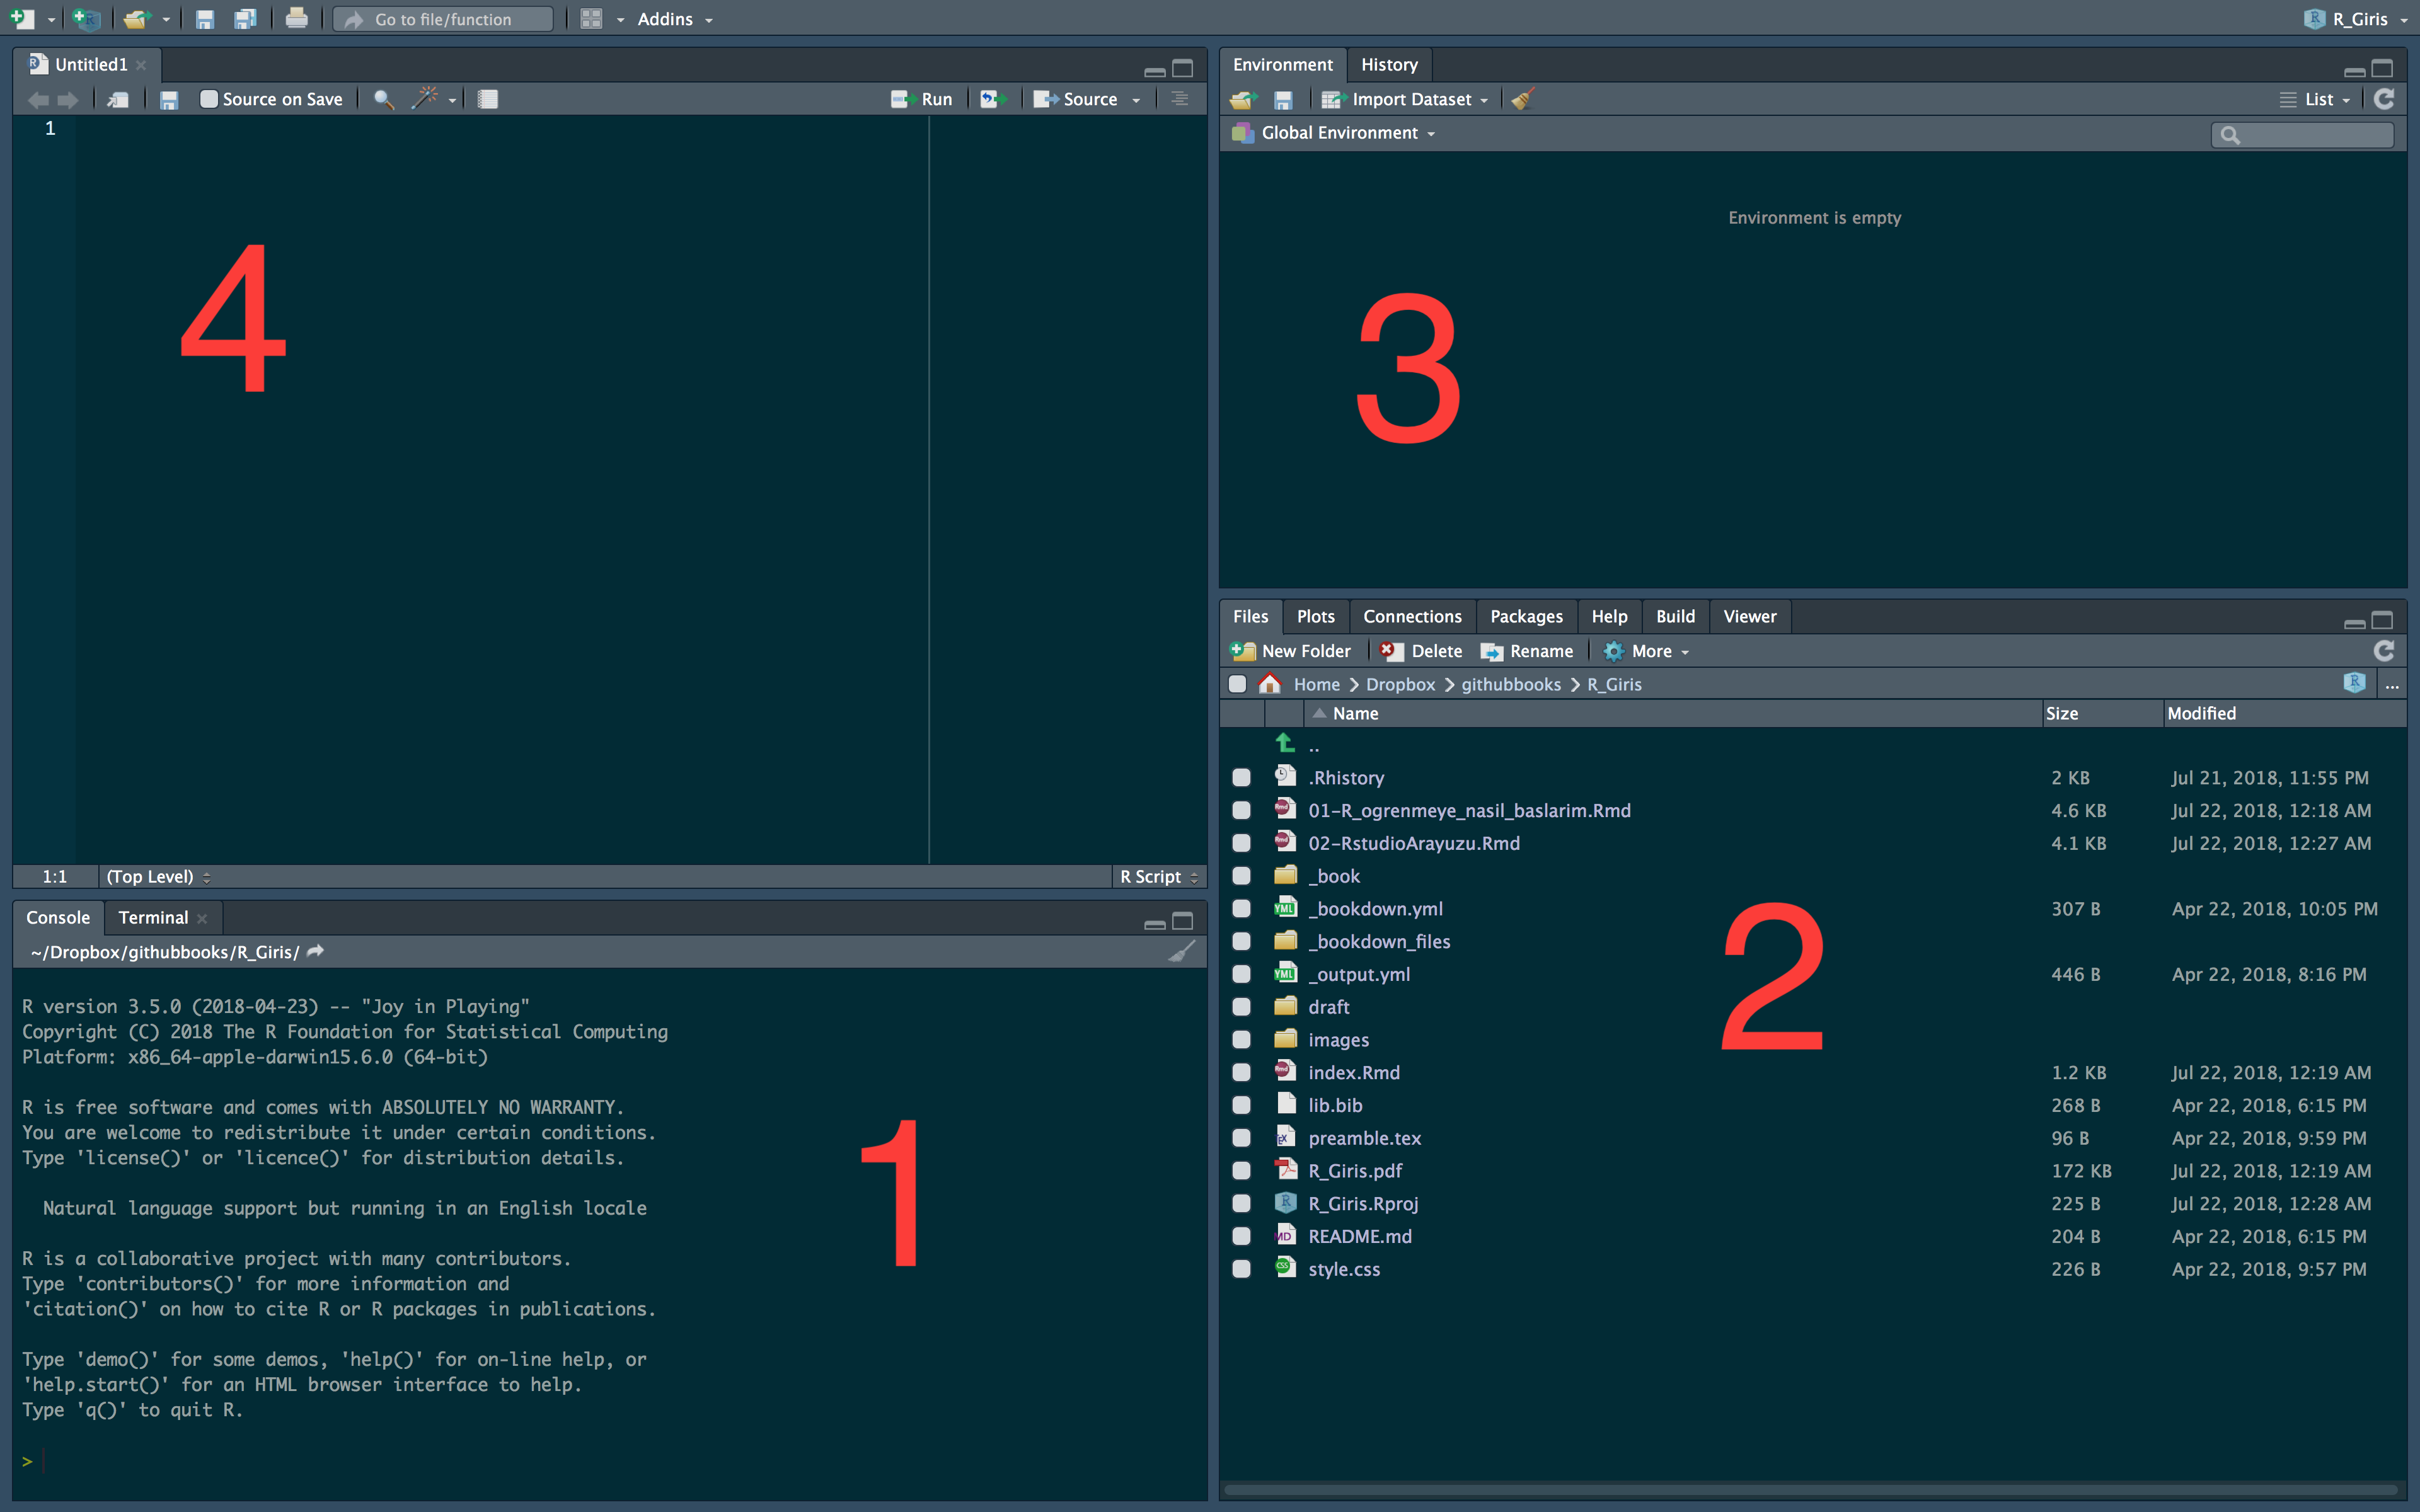
\includegraphics{images/rstudio.png}
\caption{RStudio Arayüzü}
\end{figure}

İlk olarak çalışacağımız ortamı tanıyalım.

RStudio'yu açtığınızda `RStudio Arayüzü' resmine çok benzer bir tablo
ile karşılacaksınız - belki 4. kısım hariç, oraya geleceğiz. Arkaplan
muhtemelen beyazdır ve belki işletim sistemi farkları söz konusudur. Ama
yine de bu ekran aşağı yukarı neresı ne işe yarıyor, kodu nereye
yazacağız gibi kısa bir giriş yapmak için yeterli olacaktır.

\hypertarget{konsol-terminal-1}{%
\section{Konsol, Terminal (1)}\label{konsol-terminal-1}}

\textbf{Konsol (Console)}: Burası kodu yazıp sonuçları gördüğümüz kısım.
Denemek için \texttt{2+2} yazıp enter'a basalım.

\begin{Shaded}
\begin{Highlighting}[]
\DecValTok{2} \OperatorTok{+}\StringTok{ }\DecValTok{2}
\end{Highlighting}
\end{Shaded}

\begin{verbatim}
## [1] 4
\end{verbatim}

\textbf{Terminal}: Burası da bilgisayarınızın terminali veya komut
istemcisine erişim sağlayan bir kısım. RStudio'nun eski versiyonlarında
bu özellik yoktu ancak yeni versiyon kullanıyorsanız bu sekme de mevcut
olacaktır.

\hypertarget{dosyalar-cizimler-paketler-yardm-2}{%
\section{Dosyalar, Çizimler, Paketler, Yardım
(2)}\label{dosyalar-cizimler-paketler-yardm-2}}

\textbf{Dosyalar (Files)}: İçinde bulunduğumuz klasörün içindeki
dosyaları listeliyor.

\textbf{Çizimler (Plots)}: Çizdiğimiz grafikleri görüntüleyebileceğimiz
kısım. Örneğin şu kodu konsola yazarak bu sekmenin işlevini
gözlemleyebiliriz:

\begin{Shaded}
\begin{Highlighting}[]
\KeywordTok{hist}\NormalTok{(}\KeywordTok{rnorm}\NormalTok{(}\DecValTok{1000}\NormalTok{))}
\end{Highlighting}
\end{Shaded}

\begin{figure}
\centering
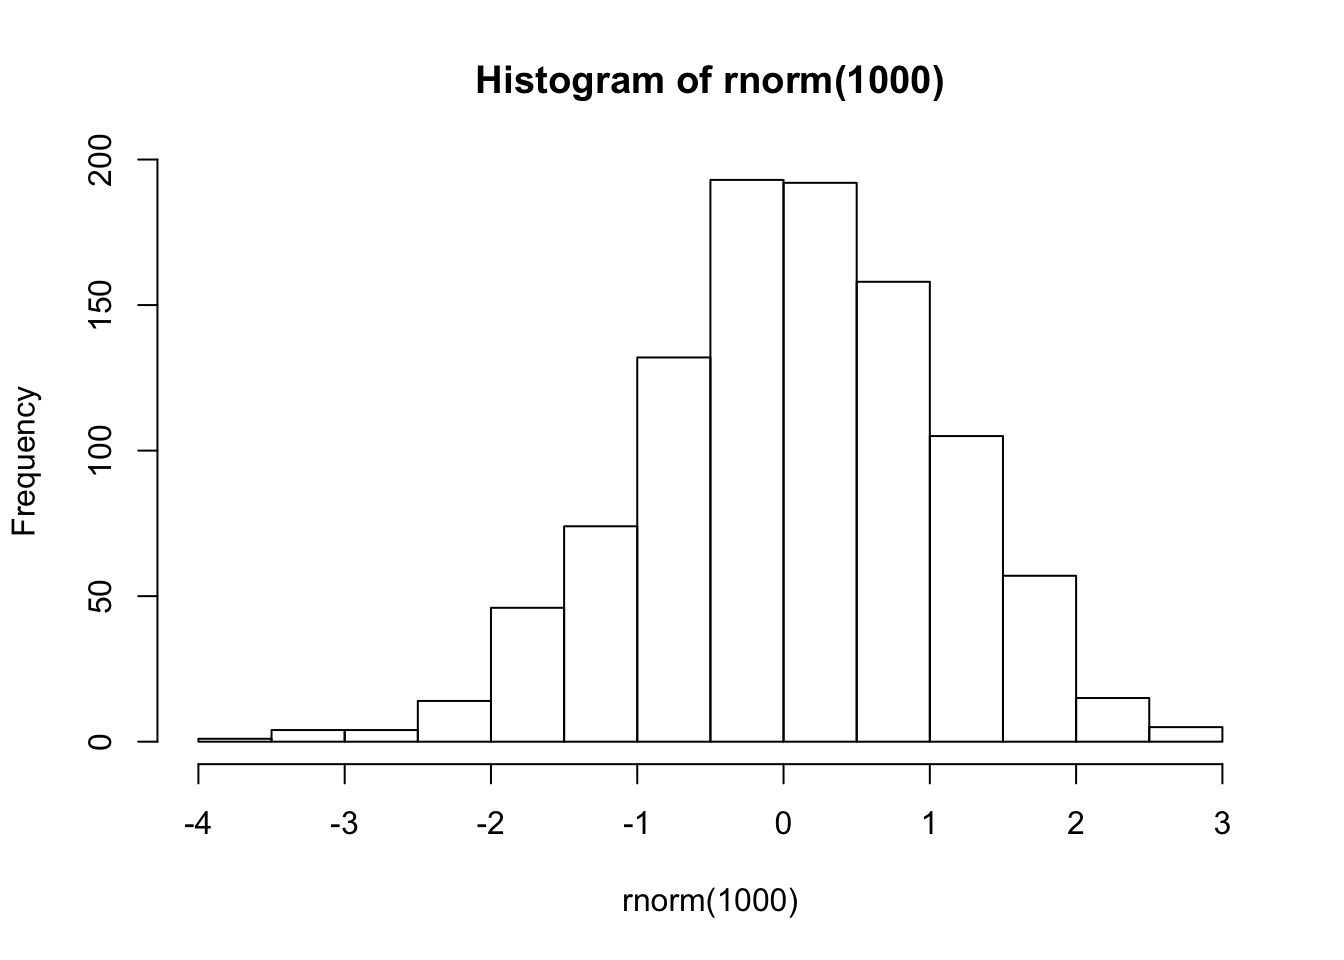
\includegraphics{R_Giris_files/figure-latex/inithist-1.pdf}
\caption{\label{fig:inithist}1000 rastgele değer kullanılarak çizilmiş bir
histogram}
\end{figure}

Bu ekranda büyütme, dışarı aktarma (export) gibi seçenekleri de
görüyoruz. Ancak grafikleri kaydetmek için bu dışarı aktarma seçeneğini
kullanmamayı, kaydetme işlemini de tamamen kod ile yapmayı tavsiye
ediyorum.

\textbf{Paketler (Packages)}: R'da yüklü olan çeşitli paketleri
(kütüphaneleri) görüyoruz. Ancak buradan R ortamımıza yükleme
yapmaktansa \texttt{library()} komutunu kullanmalıyız ki yazdığımız
kodlar daha sonra hem biz hem başkaları tarafından kolaylıkla
çalıştırılabilsin. Bu kısma sonra geleceğim.

\textbf{Yardım (Help)}: Bu sekme RStudio'daki en büyük dostumuz. Açıp
öğrenme linklerini kurcalamak iyi bir başlangıç. Ayrıca \texttt{?}
operatörü ile burada fonksiyonların yardım sayfalarını
görüntüleyebiliriz, örneğin konsolda şu kodu deneyelim:

\begin{Shaded}
\begin{Highlighting}[]
\NormalTok{?hist}
\end{Highlighting}
\end{Shaded}

Gördüğünüz gibi, yardım sekmesinde az önce histogram çizmek için
kullandığınız \texttt{hist()} fonksiyonu için yardım ekranı açıldı. Bu
ekranda, fonksiyonun tanımı, argümanları, sonucu hakkında bilgi
alabiliyor ve en altta örnekleri görüyorsunuz. Örnekleri çalıştırıp,
fonksiyonla ilgili daha fazla bilgi sahibi olabilirsiniz. Burada çıkan
bilgiler, R'ı yüklediğimizde gelen `base R' fonksiyonları için epey
detaylı. İndireceğiniz bir çok paket için de detaylı bilgi
bulabilirsiniz ancak detay ve örnek miktarı paket yazarlarının
oluşturduğu yardım dosyalarına bağlı olan bir şey.

\hypertarget{ortam-gecmis-3}{%
\section{Ortam, Geçmiş (3)}\label{ortam-gecmis-3}}

\textbf{Ortam (Environment)}: Oluşturduğumuz değişkenlerin listesini ve
bilgilerini burada görebiliriz. Şunu deneyelim:

\begin{Shaded}
\begin{Highlighting}[]
\NormalTok{x <-}\StringTok{ }\DecValTok{3}
\end{Highlighting}
\end{Shaded}

Bu kod ile, x isimli değişkene, 3 değerini vermiş olduk. Artık sadece x
yazıp enter'a basarsanız, x'in 3 olduğunu göreceksiniz. Aynı zamanda
ortam sekmesinde artık x'in de listelendiğini görebilirsiniz.

\textbf{Geçmiş (History)}: Mevcut R oturumunuzda yazdığınız kodları
listeleyen bir kısım. Buradan önceden çalıştırdığınız kodları
görebilirsiniz. Ancak daha pratik, daha çok kullanılan bir kısa yol,
konsolda iken klavyedeki yukarı ok tuşu ile önceki kodları tekrar
çağırmak. Geçmiş sadece açık oturumdaki kodları kaydediyor olsa da,
.Rhistory dosyası sayesinde ortamlar arası geçmiş bilgisini
aktarabilirsiniz. Yine de buna bağlı kalmak yerine daha sonra tekrar
kullanacağımız kodları .R scripti olarak kaydetmek çok daha elverişli
olacaktır.

\hypertarget{editor-4}{%
\section{Editör (4)}\label{editor-4}}

Editör ekranı, kodlarımızı yazıp çalıştırabileceğimiz ve sonrası için
yorumlarımızla beraber kaydedebileceğimiz ekran. Bu bölüm muhtemelen
açık olarak başlamamıştır RStudio. Burayı açmak için, sol üst köşedeki
tuş ile yeni `R script'i açabilirsiniz. Burada başka seçenekler de var,
bunların ne olduğu avantajşarı hakkında sonrasında kısımlar gelecek.
Şimdilik 'R script'ini seçelim. Açtığınız zaman, görüntüdeki gibi boş
bir bölüm çıkacak. Önerim kodlarınızı her zaman konsol yerine burada
yazmanız. RStudio'nun güzel bir özelliği burada yazdığını kodu konsolda
kolay bir şekilde çalıştırmanızı sağlıyor, kopyala yapıştır yapmanıza
gerek yok. Şimdi bu ekranda 2+2 yazıp, enter'a basalım. Konsolda hiç bir
şey olmadığını göreceksiniz. Şimdi tekrar 2+2 nin olduğu satıra dönüp
Ctrl+Enter (Mac kullanıyorsanız Cmd+Enter)'a basın. Konsolda hem kodun
çalıştırıldığını hem de sonucun burada görüntülendiğini göreceksiniz
(Eğer olmadıysa R Scripti seçeneğini seçmemiş olabilirsiniz). Her
çalışma sonunda bu dosyayı kaydederseniz (Ctrl+S ya da Cmd+S), daha
sonra yazdığınız kodlara tekrar dönme şansınız olacaktır. Daha önemlisi,
buraya yazdığınız kodların içinden hatalı olanları silebilir
düzenleyebilirsiniz bu sayede sadece işlevsel kodlarınız kaydolur.
Geleneksel olarak scriptlerin uzantıları'.R'dır.

Bu açıkladığım panellerin yeri, sırası ve açık olup olmayacağı
seçeneklerden değiştirilebilir.

Son olarak, RStudio'yu kapatırken size 'workspace'i kaydetmek isteyip
istemediğinizi soracaktır. Buna benim önerim her zaman hayır demeniz,
hatta seçeneklerden bunu varsayılan olarak ayarlayıp asla kaydetmemeniz.
Objeleri ayrıca istediğimiz şekilde nasıl kaydedeceğimizi ilerde
göreceğiz. Yine aynı şekilde history kaydetmek yerine scriptinizi
kaydetmenizi ya da history kaydetseniz bile ayrıca mutlaka scriptinizi
kaydetmenizi öneririm.

\hypertarget{ilkadimlar}{%
\chapter{İlk Adımlar}\label{ilkadimlar}}

Her zaman kod yazmaya başlamadan önce, en önemli basamak çalıştığımız
klasörün ne olduğunu bilmek, gerekirse değiştirmek.

Hangi klasörde çalıştığımızı öğrenmek için \texttt{getwd()} fonksiyonunu
kullanabiliriz (get working directory). Çalıştığımız klasörü belirlemek
içinse \texttt{setwd()} fonksiyonu kullanılıyor:

\begin{Shaded}
\begin{Highlighting}[]
\KeywordTok{getwd}\NormalTok{()}
\end{Highlighting}
\end{Shaded}

\begin{verbatim}
## [1] "/Users/melike/Dropbox/githubbooks/R_Giris"
\end{verbatim}

\begin{Shaded}
\begin{Highlighting}[]
\KeywordTok{setwd}\NormalTok{(}\StringTok{'~/Desktop'}\NormalTok{)}
\KeywordTok{getwd}\NormalTok{()}
\end{Highlighting}
\end{Shaded}

\begin{verbatim}
## [1] "/Users/melike/Desktop"
\end{verbatim}

Önerim, bilgisayarınızda R öğrenmek için bir klasör oluşturmanız ve
kodunuzu, kullandığınız dosyaları vs.~hep burada tutmanız. Aynı şekilde,
belirli bir amaçla R kullandığınız zaman da masaüstüne rastgele
isimlerle scriptleriniz kaydetmek yerine, düzenli bir şekilde uygun
klasörleri içeriğe dair fikir veren isimlendirmelerle ya da belirli bir
sistemle kaydetmeniz hayatınızı kolaylaştıracaktır.

\hypertarget{hesap-makinesi-olarak-r}{%
\section{Hesap Makinesi olarak R}\label{hesap-makinesi-olarak-r}}

En temekde hesap makinesi işlemleri yapmak için kullanabilirsiniz:

\begin{Shaded}
\begin{Highlighting}[]
\DecValTok{2}\OperatorTok{+}\DecValTok{2}
\end{Highlighting}
\end{Shaded}

\begin{verbatim}
## [1] 4
\end{verbatim}

\begin{Shaded}
\begin{Highlighting}[]
\DecValTok{2}\OperatorTok{*}\DecValTok{3}
\end{Highlighting}
\end{Shaded}

\begin{verbatim}
## [1] 6
\end{verbatim}

\begin{Shaded}
\begin{Highlighting}[]
\DecValTok{10-5}
\end{Highlighting}
\end{Shaded}

\begin{verbatim}
## [1] 5
\end{verbatim}

\begin{Shaded}
\begin{Highlighting}[]
\DecValTok{3}\OperatorTok{^}\DecValTok{2}
\end{Highlighting}
\end{Shaded}

\begin{verbatim}
## [1] 9
\end{verbatim}

\begin{Shaded}
\begin{Highlighting}[]
\DecValTok{450}\OperatorTok{/}\DecValTok{3}
\end{Highlighting}
\end{Shaded}

\begin{verbatim}
## [1] 150
\end{verbatim}

\begin{Shaded}
\begin{Highlighting}[]
\DecValTok{200}\OperatorTok{/}\DecValTok{3}
\end{Highlighting}
\end{Shaded}

\begin{verbatim}
## [1] 66.66667
\end{verbatim}

\begin{Shaded}
\begin{Highlighting}[]
\DecValTok{200}\OperatorTok\DecValTok{3}
\end{Highlighting}
\end{Shaded}

\begin{verbatim}
## [1] 2
\end{verbatim}

\begin{Shaded}
\begin{Highlighting}[]
\DecValTok{200}\OperatorTok\DecValTok{3}
\end{Highlighting}
\end{Shaded}

\begin{verbatim}
## [1] 66
\end{verbatim}

Çok açık olmayan operatörler:

\begin{itemize}
\tightlist
\item
  \texttt{\%\%}-- belirli bir tabanda kalan işlemi, modüler aritmetik.
  Örneğimizde 200ün 3e bölümünden kalan 2
\item
  \texttt{\%/\%} -- tam sayı bölmesi, kalan olsa bile tam sayı olarak
  bölme işleminin sonucu
\end{itemize}

\hypertarget{fonksiyonlar}{%
\section{Fonksiyonlar}\label{fonksiyonlar}}

R kendi içinde fonksiyonlar barındırır. Örneğin, başlangıçta
kullandığımız \texttt{getwd()} gibi. Farkettiysenz, fonksiyonlardan
bahsederken hep parantez kullanıyorum. Fonksiyonları değişkenlerden
ayırabileceğiniz en basit şekil bu. Çok basit bir kaç fonksiyona
bakalım:

\begin{Shaded}
\begin{Highlighting}[]
\CommentTok{#10 tabaninda log}
\KeywordTok{log10}\NormalTok{(}\DecValTok{100}\NormalTok{) }
\end{Highlighting}
\end{Shaded}

\begin{verbatim}
## [1] 2
\end{verbatim}

\begin{Shaded}
\begin{Highlighting}[]
\CommentTok{#2 tabaninda log}
\KeywordTok{log2}\NormalTok{(}\DecValTok{100}\NormalTok{)}
\end{Highlighting}
\end{Shaded}

\begin{verbatim}
## [1] 6.643856
\end{verbatim}

\begin{Shaded}
\begin{Highlighting}[]
\CommentTok{#4 tabaninda 10un log'u}
\KeywordTok{log}\NormalTok{(}\DecValTok{10}\NormalTok{,}\DecValTok{4}\NormalTok{) }
\end{Highlighting}
\end{Shaded}

\begin{verbatim}
## [1] 1.660964
\end{verbatim}

\begin{Shaded}
\begin{Highlighting}[]
\CommentTok{#e uzeri 1}
\KeywordTok{exp}\NormalTok{(}\DecValTok{1}\NormalTok{) }
\end{Highlighting}
\end{Shaded}

\begin{verbatim}
## [1] 2.718282
\end{verbatim}

\begin{Shaded}
\begin{Highlighting}[]
\CommentTok{# e uzeri 2}
\KeywordTok{exp}\NormalTok{(}\DecValTok{2}\NormalTok{) }
\end{Highlighting}
\end{Shaded}

\begin{verbatim}
## [1] 7.389056
\end{verbatim}

\begin{Shaded}
\begin{Highlighting}[]
 \CommentTok{# e uzeri 2 nin ln i - log taban belirtilmediginde e tabaninda islem yapar}
\KeywordTok{log}\NormalTok{(}\KeywordTok{exp}\NormalTok{(}\DecValTok{2}\NormalTok{))}
\end{Highlighting}
\end{Shaded}

\begin{verbatim}
## [1] 2
\end{verbatim}

\begin{Shaded}
\begin{Highlighting}[]
\CommentTok{# 16 nin koku}
\DecValTok{16}\OperatorTok{^}\NormalTok{(}\DecValTok{1}\OperatorTok{/}\DecValTok{2}\NormalTok{)}
\end{Highlighting}
\end{Shaded}

\begin{verbatim}
## [1] 4
\end{verbatim}

\begin{Shaded}
\begin{Highlighting}[]
\CommentTok{# ayni islem fonksiyon ile}
\KeywordTok{sqrt}\NormalTok{(}\DecValTok{16}\NormalTok{) }
\end{Highlighting}
\end{Shaded}

\begin{verbatim}
## [1] 4
\end{verbatim}

\hypertarget{rda-degiskenler}{%
\section{R'da değişkenler}\label{rda-degiskenler}}

Değişkenler, veri tutucular olarak düşünülebilir. R'da değişkene değer
atamak icin \texttt{=} veya \texttt{\textless{}-} operatörleri
kullanılabilir. Örneğin x'e 3 değerini atamak için, aşağıdaki iki kod da
geçerlidir.

\begin{Shaded}
\begin{Highlighting}[]
\NormalTok{x =}\StringTok{ }\DecValTok{3}
\NormalTok{x}
\end{Highlighting}
\end{Shaded}

\begin{verbatim}
## [1] 3
\end{verbatim}

\begin{Shaded}
\begin{Highlighting}[]
\NormalTok{a <-}\StringTok{ }\DecValTok{4}
\NormalTok{a}
\end{Highlighting}
\end{Shaded}

\begin{verbatim}
## [1] 4
\end{verbatim}

\begin{Shaded}
\begin{Highlighting}[]
\DecValTok{3} \OperatorTok{*}\StringTok{ }\DecValTok{4}
\end{Highlighting}
\end{Shaded}

\begin{verbatim}
## [1] 12
\end{verbatim}

\begin{Shaded}
\begin{Highlighting}[]
\NormalTok{x }\OperatorTok{*}\StringTok{ }\NormalTok{a}
\end{Highlighting}
\end{Shaded}

\begin{verbatim}
## [1] 12
\end{verbatim}

\texttt{\textless{}-} tarihsel olarak R camiasında çokça kullanılsa da,
pratik nedenlerle \texttt{=} kullanımı da oldukça yaygın ve yanlış
değildir.

\hypertarget{degisken-isimleri}{%
\subsection{Değişken isimleri}\label{degisken-isimleri}}

R'da değişkenlere verebileceğimiz isimler için bazı sınırlayıcı kurallar
vardır. Değişkenler, bir harf ile ya da harfin takip ettiği nokta ile
başlar. Öğrneğin, \texttt{benimdegiskenim} geçerli bir değişken isim
iken \texttt{2değisken} geçerli değildir, çünkü 2 bir harf değildir.
\texttt{.degisken} geçerli bir değişken ismidir ancak
\texttt{.2degisken} değildir. Ayrıca R'da kimi özel anlam içeren
keilemerin değişken olarak kullanılması mümkün değildir, \texttt{ìf} ve
\texttt{for} gibi. Bunları \texttt{?reserved} yazarak öğrenebilirsiniz.

Yasak olmasa da diğer bir sorun R içinde varolan fonksiyonların isimleri
ile değişken yaratmak. Çoğu zaman sorun olmadan çalışsa bile,
karışıklığa sebep olduğu durumlar olabilir.

R'da değişken isimleri küçük / büyük harfe duyarlıdır.

Değişken isimlerini tuttuğu veriyle alakalı seçmek kolaylık sağlar.

\hypertarget{temel-obje-turleri}{%
\chapter{Temel obje türleri}\label{temel-obje-turleri}}

R'da 5 çeşit temel obje türü var:

\hypertarget{karakter-character}{%
\section{Karakter (character)}\label{karakter-character}}

\begin{Shaded}
\begin{Highlighting}[]
\NormalTok{x =}\StringTok{ 'a'}
\NormalTok{x}
\end{Highlighting}
\end{Shaded}

\begin{verbatim}
## [1] "a"
\end{verbatim}

\begin{Shaded}
\begin{Highlighting}[]
\NormalTok{a}
\end{Highlighting}
\end{Shaded}

\begin{verbatim}
## [1] 4
\end{verbatim}

Karakter değişkeni yaratmak için, tırnak işaretlerini
(\texttt{\textquotesingle{}\textquotesingle{}}) kullanıyoruz. Yani,
\texttt{x} bir obje iken \texttt{\textquotesingle{}a\textquotesingle{}}
bir karakterdir. Bu sebeple, \texttt{a} yazdığınızda, R \texttt{a}
isminde bir obje arıyor, bizim a isminde bir objemiz olmadığından
\texttt{obje\ bulunamadı} hatası veriyor. Bu arada R'da en iyi dostumuz
hata mesajları. Genelde hata mesajı sorunun nerede olduğu hakkında çok
iyi fikir verecektir.

\begin{Shaded}
\begin{Highlighting}[]
\KeywordTok{class}\NormalTok{(x)}
\end{Highlighting}
\end{Shaded}

\begin{verbatim}
## [1] "character"
\end{verbatim}

\texttt{class()} fonksiyonu obje sınıfını öğrenmemizi sağlıyor.

\begin{Shaded}
\begin{Highlighting}[]
\NormalTok{x =}\StringTok{ 'melike'}
\NormalTok{x}
\end{Highlighting}
\end{Shaded}

\begin{verbatim}
## [1] "melike"
\end{verbatim}

\begin{Shaded}
\begin{Highlighting}[]
\KeywordTok{class}\NormalTok{(x)}
\end{Highlighting}
\end{Shaded}

\begin{verbatim}
## [1] "character"
\end{verbatim}

Karakter sınıfındaki objeler, tek bir karakter içermek zorunda değil,
\texttt{\textquotesingle{}a\textquotesingle{}} da
\texttt{\textquotesingle{}aaa\textquotesingle{}} da karakter
objeleridir.

\hypertarget{numerik-numeric}{%
\section{Nümerik (numeric)}\label{numerik-numeric}}

\begin{Shaded}
\begin{Highlighting}[]
\NormalTok{x =}\StringTok{ }\DecValTok{3}
\NormalTok{x}
\end{Highlighting}
\end{Shaded}

\begin{verbatim}
## [1] 3
\end{verbatim}

\begin{Shaded}
\begin{Highlighting}[]
\KeywordTok{class}\NormalTok{(x)}
\end{Highlighting}
\end{Shaded}

\begin{verbatim}
## [1] "numeric"
\end{verbatim}

\begin{Shaded}
\begin{Highlighting}[]
\NormalTok{x =}\StringTok{ }\FloatTok{3.14}
\NormalTok{x}
\end{Highlighting}
\end{Shaded}

\begin{verbatim}
## [1] 3.14
\end{verbatim}

\begin{Shaded}
\begin{Highlighting}[]
\KeywordTok{class}\NormalTok{(x)}
\end{Highlighting}
\end{Shaded}

\begin{verbatim}
## [1] "numeric"
\end{verbatim}

\begin{Shaded}
\begin{Highlighting}[]
\NormalTok{x=}\StringTok{ }\DecValTok{1}\OperatorTok{/}\DecValTok{0}
\NormalTok{x}
\end{Highlighting}
\end{Shaded}

\begin{verbatim}
## [1] Inf
\end{verbatim}

\begin{Shaded}
\begin{Highlighting}[]
\KeywordTok{class}\NormalTok{(x)}
\end{Highlighting}
\end{Shaded}

\begin{verbatim}
## [1] "numeric"
\end{verbatim}

\begin{Shaded}
\begin{Highlighting}[]
\NormalTok{x =}\StringTok{ }\DecValTok{0} \OperatorTok{/}\StringTok{ }\DecValTok{0}
\NormalTok{x}
\end{Highlighting}
\end{Shaded}

\begin{verbatim}
## [1] NaN
\end{verbatim}

\begin{Shaded}
\begin{Highlighting}[]
\KeywordTok{class}\NormalTok{(x)}
\end{Highlighting}
\end{Shaded}

\begin{verbatim}
## [1] "numeric"
\end{verbatim}

Burada ilginç olan kısımlar:

\begin{enumerate}
\def\labelenumi{\arabic{enumi}.}
\tightlist
\item
  R tam sayıları da özellikle belirtmediğimiz sürece nümerik olarak
  alıyor
\item
  \texttt{Sonsuz}un (\texttt{Inf}) veri tipi nümerik
\item
  \texttt{NaN} (``not a number'', ``sayı değil'') değeri de nümerik
  sınıfında.
\end{enumerate}

\hypertarget{tam-saylar-integer}{%
\section{Tam sayılar (integer)}\label{tam-saylar-integer}}

\begin{Shaded}
\begin{Highlighting}[]
\NormalTok{x =}\StringTok{ }\NormalTok{3L}
\NormalTok{x}
\end{Highlighting}
\end{Shaded}

\begin{verbatim}
## [1] 3
\end{verbatim}

\begin{Shaded}
\begin{Highlighting}[]
\KeywordTok{class}\NormalTok{(x)}
\end{Highlighting}
\end{Shaded}

\begin{verbatim}
## [1] "integer"
\end{verbatim}

Özellikle tam sayı oluşturmak istiyorsak sondaki L ekini kullanmalıyız.

\hypertarget{kompleks-complex}{%
\section{Kompleks (complex)}\label{kompleks-complex}}

\begin{Shaded}
\begin{Highlighting}[]
\NormalTok{x =}\StringTok{ }\DecValTok{1}\OperatorTok{+}\NormalTok{4i}
\NormalTok{x}
\end{Highlighting}
\end{Shaded}

\begin{verbatim}
## [1] 1+4i
\end{verbatim}

\begin{Shaded}
\begin{Highlighting}[]
\KeywordTok{class}\NormalTok{(x)}
\end{Highlighting}
\end{Shaded}

\begin{verbatim}
## [1] "complex"
\end{verbatim}

\hypertarget{mantksal-logical-boolean}{%
\section{Mantıksal (logical, boolean)}\label{mantksal-logical-boolean}}

\begin{Shaded}
\begin{Highlighting}[]
\NormalTok{x =}\StringTok{ }\OtherTok{TRUE}
\NormalTok{x}
\end{Highlighting}
\end{Shaded}

\begin{verbatim}
## [1] TRUE
\end{verbatim}

\begin{Shaded}
\begin{Highlighting}[]
\KeywordTok{class}\NormalTok{(x)}
\end{Highlighting}
\end{Shaded}

\begin{verbatim}
## [1] "logical"
\end{verbatim}

\begin{Shaded}
\begin{Highlighting}[]
\NormalTok{x =}\StringTok{ }\OtherTok{FALSE}
\NormalTok{x}
\end{Highlighting}
\end{Shaded}

\begin{verbatim}
## [1] FALSE
\end{verbatim}

\begin{Shaded}
\begin{Highlighting}[]
\KeywordTok{class}\NormalTok{(x)}
\end{Highlighting}
\end{Shaded}

\begin{verbatim}
## [1] "logical"
\end{verbatim}

\begin{Shaded}
\begin{Highlighting}[]
\NormalTok{x =}\StringTok{ }\NormalTok{T}
\NormalTok{x}
\end{Highlighting}
\end{Shaded}

\begin{verbatim}
## [1] TRUE
\end{verbatim}

TRUE ve FALSE iki temel mantıksal değişken (True=Doğru, False=Yanlış).
Sadece baş harfleri kullanılarak da ifade edilebilirler.

\begin{Shaded}
\begin{Highlighting}[]
\NormalTok{x =}\StringTok{ }\NormalTok{f}
\end{Highlighting}
\end{Shaded}

\begin{verbatim}
## Error in eval(expr, envir, enclos): object 'f' not found
\end{verbatim}

Ancak bu harfler büyük harf olmali yoksa \texttt{f} ismindeki objeye
eşitlemeye çalışmış oluyoruz x'i.

Alıştırma olarak şu objelerin sınıflarını tahmin etmeye çalışıp, yanılıp
yanılmadığınızı kontrol edebilirsiniz:

\begin{Shaded}
\begin{Highlighting}[]
\NormalTok{a=}\StringTok{'5'} 
\NormalTok{b=}\StringTok{'T'}
\NormalTok{y=}\FloatTok{10.5}\NormalTok{L}
\NormalTok{x=}\StringTok{'y'}
\NormalTok{d=x}
\end{Highlighting}
\end{Shaded}

Tırnak işaretleri içinde veriler girildiğinden \texttt{a}, \texttt{b},
\texttt{x}, ve dolayısıyla \texttt{d} objeleri karakter tipindedir.
\texttt{y} ise ondalıklı değer girdiğimizden \texttt{L} uzantısını
kullansak da tam sayı değil nümerik tipindedir.

İlerledikçe \texttt{class()} fonksiyonu ile objelere baktığınızda farklı
cevaplar alacağız. Mesela objelerden oluşan objelerimiz olduğunda - 1den
100e kadar olan sayıları içeren 10x10luk bir matrisiniz varsa mesela
(\texttt{class(matrix(1:100,10))}). Veya R'ın nesne tabalı programlama
(object oriented programming) dili olmasının getirisi olarak, yeni obje
sınıfları ile çalıştığınızda.

Eğer ki obje açık bir obje sınıfına sahipse (örn. matrix gibi), nümerik
değerlerden oluşan bir obje mi, karakter objesi mi, bunu görmek yerine
sınıfını göreceksiniz. Bu durumda \texttt{mode()} fonksiyonunu
kullanarak ne tip objelerden oluştuğunu görebiliriz, örn
\texttt{mode(matrix(1:100,10))}.

\hypertarget{vektorler}{%
\chapter{Vektörler}\label{vektorler}}

R kimi veri yapıları üzerinde işlem yapar. En basit veri yapılarından
biri olan vektörler, aynı temel obje türünden öğeler içeren dizilerdir.

\begin{Shaded}
\begin{Highlighting}[]
\NormalTok{x =}\StringTok{ }\KeywordTok{c}\NormalTok{(}\DecValTok{1}\NormalTok{,}\DecValTok{2}\NormalTok{,}\DecValTok{3}\NormalTok{)}
\NormalTok{x}
\end{Highlighting}
\end{Shaded}

\begin{verbatim}
## [1] 1 2 3
\end{verbatim}

Burada `x'; 1, 2, ve 3 öğelerine sahip bir vektördür. Vektör oluşturmak
için bu örnekte \texttt{c()} fonksiyonunu kullandık. \texttt{c}yi,
\texttt{concatenate} (bağlamak) ya da \texttt{combine} (birleştirmek)
kelimelerinden birinin kısaltılmış hali olarak aklınızda tutabilirsiniz.

Önceki örnekte nümerik tipte öğelerden oluşan bir vektör yarattık. Ancak
vektörler hepsi aynı olduğu sürece diğer tiplerden de oluşabilir.

\begin{Shaded}
\begin{Highlighting}[]
\NormalTok{x =}\StringTok{ }\KeywordTok{c}\NormalTok{(T,F,F) }\CommentTok{# logical}
\NormalTok{x}
\end{Highlighting}
\end{Shaded}

\begin{verbatim}
## [1]  TRUE FALSE FALSE
\end{verbatim}

\begin{Shaded}
\begin{Highlighting}[]
\NormalTok{x =}\StringTok{ }\KeywordTok{c}\NormalTok{(}\StringTok{'x'}\NormalTok{,}\StringTok{'y'}\NormalTok{,}\StringTok{'aa'}\NormalTok{,}\StringTok{'oiasjfioasjf'}\NormalTok{) }\CommentTok{# character}
\NormalTok{x}
\end{Highlighting}
\end{Shaded}

\begin{verbatim}
## [1] "x"            "y"            "aa"           "oiasjfioasjf"
\end{verbatim}

\begin{Shaded}
\begin{Highlighting}[]
\NormalTok{x =}\StringTok{ }\KeywordTok{c}\NormalTok{(}\DecValTok{1}\OperatorTok{+}\NormalTok{4i,}\DecValTok{5}\OperatorTok{+}\NormalTok{2i) }\CommentTok{# complex}
\NormalTok{x}
\end{Highlighting}
\end{Shaded}

\begin{verbatim}
## [1] 1+4i 5+2i
\end{verbatim}

\begin{Shaded}
\begin{Highlighting}[]
\NormalTok{x =}\StringTok{ }\KeywordTok{c}\NormalTok{(1L,5L) }\CommentTok{#integer}
\NormalTok{x}
\end{Highlighting}
\end{Shaded}

\begin{verbatim}
## [1] 1 5
\end{verbatim}

Şimdi de aynı tipte olmayan öğelerle vektör oluşturmaya çalıştığımızda
ne oluyor, bunu görelim. İlk deneme olarak bütün tipleri girdi olarak
verip bir vektör yaratmaya çalışalım.

\begin{Shaded}
\begin{Highlighting}[]
\NormalTok{x =}\StringTok{ }\KeywordTok{c}\NormalTok{(}\FloatTok{1.5}\NormalTok{, }\StringTok{'karakter'}\NormalTok{, 3i}\OperatorTok{+}\DecValTok{2}\NormalTok{, }\OtherTok{TRUE}\NormalTok{, F)}
\end{Highlighting}
\end{Shaded}

Bu örnekte; nümerik, karakter, kompleks ve boolean tipinde öğelerle ile
bir vektor yaratmak istedik. Ve hata almadık Peki `x' objesinin modu ne
ve nasıl bir vektor elde ettik?

\begin{Shaded}
\begin{Highlighting}[]
\NormalTok{x}
\end{Highlighting}
\end{Shaded}

\begin{verbatim}
## [1] "1.5"      "karakter" "2+3i"     "TRUE"     "FALSE"
\end{verbatim}

Hata almadık ama vektör oluşturma sırasında öğeler kendi modlarını
koruyamadılar. Data tipleri arasında bir hiyerarşi vardır ve R farklı
tipte öğeleri birleştirirken bu objelerde hiyerarşide en yüksek olanı
seçerek vektör yaratır. Buradan yapacağımız çıkarım, karakter tipi
hiyerarşide en yüksek olan. Şimdi sırasıyla en yüksekte olanı çıkartarak
hiyerarşiyi çözmeye çalışalım.

\begin{Shaded}
\begin{Highlighting}[]
\CommentTok{# karakteri cikarttigimizda}
\NormalTok{x =}\StringTok{ }\KeywordTok{c}\NormalTok{(}\FloatTok{1.5}\NormalTok{, 3i}\OperatorTok{+}\DecValTok{2}\NormalTok{, }\OtherTok{TRUE}\NormalTok{, F)}
\KeywordTok{mode}\NormalTok{(x)}
\end{Highlighting}
\end{Shaded}

\begin{verbatim}
## [1] "complex"
\end{verbatim}

\begin{Shaded}
\begin{Highlighting}[]
\NormalTok{x }
\end{Highlighting}
\end{Shaded}

\begin{verbatim}
## [1] 1.5+0i 2.0+3i 1.0+0i 0.0+0i
\end{verbatim}

\begin{Shaded}
\begin{Highlighting}[]
\CommentTok{# kompleksi cikarttigimizda}
\NormalTok{x =}\StringTok{ }\KeywordTok{c}\NormalTok{(}\FloatTok{1.5}\NormalTok{, }\OtherTok{TRUE}\NormalTok{, F)}
\KeywordTok{mode}\NormalTok{(x)}
\end{Highlighting}
\end{Shaded}

\begin{verbatim}
## [1] "numeric"
\end{verbatim}

\begin{Shaded}
\begin{Highlighting}[]
\NormalTok{x}
\end{Highlighting}
\end{Shaded}

\begin{verbatim}
## [1] 1.5 1.0 0.0
\end{verbatim}

\begin{Shaded}
\begin{Highlighting}[]
\CommentTok{# numerigi cikarttigimizda}
\NormalTok{x =}\StringTok{ }\KeywordTok{c}\NormalTok{(}\OtherTok{TRUE}\NormalTok{, F)}
\KeywordTok{mode}\NormalTok{(x)}
\end{Highlighting}
\end{Shaded}

\begin{verbatim}
## [1] "logical"
\end{verbatim}

\begin{Shaded}
\begin{Highlighting}[]
\NormalTok{x}
\end{Highlighting}
\end{Shaded}

\begin{verbatim}
## [1]  TRUE FALSE
\end{verbatim}

Bu durumda boolean \textless{} nümerik \textless{} kompleks \textless{}
karakter çıkarımını yapabiliriz.

\hypertarget{vektorleri-birlestirmek}{%
\section{Vektorleri birleştirmek}\label{vektorleri-birlestirmek}}

Vektör yaratmak için kullandığımız c() fonksiyonu, aynı zamanda
vektörleri birleştirmek için de kullanılabilir.

\begin{Shaded}
\begin{Highlighting}[]
\NormalTok{x =}\StringTok{ }\KeywordTok{c}\NormalTok{(}\DecValTok{1}\NormalTok{,}\DecValTok{2}\NormalTok{,}\DecValTok{3}\NormalTok{)}
\NormalTok{x}
\end{Highlighting}
\end{Shaded}

\begin{verbatim}
## [1] 1 2 3
\end{verbatim}

\begin{Shaded}
\begin{Highlighting}[]
\NormalTok{y =}\StringTok{ }\KeywordTok{c}\NormalTok{(}\DecValTok{4}\NormalTok{,}\DecValTok{5}\NormalTok{,}\DecValTok{6}\NormalTok{)}
\NormalTok{y}
\end{Highlighting}
\end{Shaded}

\begin{verbatim}
## [1] 4 5 6
\end{verbatim}

\begin{Shaded}
\begin{Highlighting}[]
\NormalTok{z =}\StringTok{ }\KeywordTok{c}\NormalTok{(x,y)}
\NormalTok{z}
\end{Highlighting}
\end{Shaded}

\begin{verbatim}
## [1] 1 2 3 4 5 6
\end{verbatim}

\begin{Shaded}
\begin{Highlighting}[]
\NormalTok{a =}\StringTok{ }\KeywordTok{c}\NormalTok{(z,}\DecValTok{9}\NormalTok{,}\DecValTok{8}\NormalTok{)}
\NormalTok{a}
\end{Highlighting}
\end{Shaded}

\begin{verbatim}
## [1] 1 2 3 4 5 6 9 8
\end{verbatim}

Ve önceden bahsettiğimiz, data tipinin hiyerarşide en yüksek olana
dönüştürülmesi bu durumda da geçerlidir.

\begin{Shaded}
\begin{Highlighting}[]
\NormalTok{x =}\StringTok{ }\KeywordTok{c}\NormalTok{(}\DecValTok{1}\NormalTok{,}\DecValTok{2}\NormalTok{,}\DecValTok{3}\NormalTok{)}
\NormalTok{x}
\end{Highlighting}
\end{Shaded}

\begin{verbatim}
## [1] 1 2 3
\end{verbatim}

\begin{Shaded}
\begin{Highlighting}[]
\NormalTok{y =}\StringTok{ }\KeywordTok{c}\NormalTok{(}\StringTok{'a'}\NormalTok{,}\StringTok{'b'}\NormalTok{,}\StringTok{'c'}\NormalTok{)}
\NormalTok{y}
\end{Highlighting}
\end{Shaded}

\begin{verbatim}
## [1] "a" "b" "c"
\end{verbatim}

\begin{Shaded}
\begin{Highlighting}[]
\NormalTok{z =}\StringTok{ }\KeywordTok{c}\NormalTok{(x,y)}
\NormalTok{z}
\end{Highlighting}
\end{Shaded}

\begin{verbatim}
## [1] "1" "2" "3" "a" "b" "c"
\end{verbatim}

\hypertarget{vektor-aritmetigi}{%
\section{Vektor aritmetiği}\label{vektor-aritmetigi}}

Daha önce R'ı hesap makinesi gibi kullanabileceğimizi görmüştük.
Vektörlerle de aynı işlemleri yapabilirsiniz.

\begin{Shaded}
\begin{Highlighting}[]
\NormalTok{x =}\StringTok{ }\KeywordTok{c}\NormalTok{(}\DecValTok{1}\NormalTok{,}\DecValTok{2}\NormalTok{,}\DecValTok{3}\NormalTok{)}
\NormalTok{x }\OperatorTok{*}\StringTok{ }\DecValTok{3}
\end{Highlighting}
\end{Shaded}

\begin{verbatim}
## [1] 3 6 9
\end{verbatim}

\begin{Shaded}
\begin{Highlighting}[]
\NormalTok{x }\OperatorTok{+}\StringTok{ }\DecValTok{1}
\end{Highlighting}
\end{Shaded}

\begin{verbatim}
## [1] 2 3 4
\end{verbatim}

\begin{Shaded}
\begin{Highlighting}[]
\NormalTok{(x }\OperatorTok{*}\StringTok{ }\DecValTok{5}\NormalTok{) }\DecValTok{-2}
\end{Highlighting}
\end{Shaded}

\begin{verbatim}
## [1]  3  8 13
\end{verbatim}

Burada önemli olan, işlemlerin her bir öğe üzerinde ayrı ayrı
gerçekleştiriliyor oluşu. Eğer iki vektörümüz olsaydı,ve bu iki vektörü
toplamak isteseysdik, benzer şekilde birinci öğenin ikinci vektördeki
birinci öğe ile, ikinci öğenin ikinci vektördeki ikinci öğe ile vb.
şekilde toplandığını görürdük.

\begin{Shaded}
\begin{Highlighting}[]
\NormalTok{x =}\StringTok{ }\KeywordTok{c}\NormalTok{(}\DecValTok{1}\NormalTok{,}\DecValTok{2}\NormalTok{,}\DecValTok{3}\NormalTok{)}
\NormalTok{y =}\StringTok{ }\KeywordTok{c}\NormalTok{(}\DecValTok{4}\NormalTok{,}\DecValTok{5}\NormalTok{,}\DecValTok{6}\NormalTok{)}
\NormalTok{x }\OperatorTok{+}\StringTok{ }\NormalTok{y}
\end{Highlighting}
\end{Shaded}

\begin{verbatim}
## [1] 5 7 9
\end{verbatim}

\begin{Shaded}
\begin{Highlighting}[]
\NormalTok{x }\OperatorTok{*}\StringTok{ }\NormalTok{y}
\end{Highlighting}
\end{Shaded}

\begin{verbatim}
## [1]  4 10 18
\end{verbatim}

Peki ya vektörlerimi eşit uzunlukta değilse? Bu durumda kısa olan
vektor, uzun vektordeki öğeler bitene kadar tekrar tekrar kullanılır.

\begin{Shaded}
\begin{Highlighting}[]
\NormalTok{x =}\StringTok{ }\KeywordTok{c}\NormalTok{(}\DecValTok{1}\NormalTok{,}\DecValTok{2}\NormalTok{,}\DecValTok{3}\NormalTok{,}\DecValTok{4}\NormalTok{)}
\NormalTok{y =}\StringTok{ }\KeywordTok{c}\NormalTok{(}\DecValTok{2}\NormalTok{,}\DecValTok{3}\NormalTok{)}
\NormalTok{x }\OperatorTok{*}\StringTok{ }\NormalTok{y}
\end{Highlighting}
\end{Shaded}

\begin{verbatim}
## [1]  2  6  6 12
\end{verbatim}

\begin{itemize}
\tightlist
\item
  İlk vektördeki ilk eleman olan 1, ikinci vektördeki ilk eleman olan 2
  ile çarpıldı ve sonucun ilk elemanı 2 oldu.
\item
  İlk vektördeki ikinci eleman olan 2, ikinci vektördeki ikinci eleman
  olan 3 ile çarğıldı ve sonucun ikinci elemanı 6 oldu.
\item
  İlk vektördeki üçüncü eleman olan 3, ikinci vektörde üçüncü bir eleman
  olmamasından dolayı ilk eleman olan 2 ile çarpıldı ve sonucun üçüncü
  elemanı 6 oldu.
\item
  İlk vektördeki dördüncü eleman olan 4, ikinci vektörde ikinci eleman
  olan 3 ile çarpıldı ve sonucun üçüncü elemanı 12 oldu.
\end{itemize}

Yani bu tarz işlemleri yaparken dikkat etmek gerekiyor. Bu işlemin
sonucunda R'ın nasıl davranacağını bilmeyen birisi 8 elemanlı bir vektör
almayı, yani ilk vektör önce 2 sonra 3 ile çarpıp birleştirilir diye
bekleyebilir örneğin. Ancak R böyle davranmıyor.

Peki ya vektörlerimizin uzunluğu birbirinin katı olmasaydı? Burada 4
öğeli bir vektörü 2 öğeli bir vektör ile çarptık. 4 öğeli bir vektörü, 3
öğeli bir vektör ile çarpmaya çalışsaydık farklı bir davranış bekler
miyiz?

\begin{Shaded}
\begin{Highlighting}[]
\NormalTok{x =}\StringTok{ }\KeywordTok{c}\NormalTok{(}\DecValTok{1}\NormalTok{,}\DecValTok{2}\NormalTok{,}\DecValTok{3}\NormalTok{,}\DecValTok{4}\NormalTok{)}
\NormalTok{y =}\StringTok{ }\KeywordTok{c}\NormalTok{(}\DecValTok{1}\NormalTok{,}\DecValTok{2}\NormalTok{,}\DecValTok{3}\NormalTok{)}
\NormalTok{x }\OperatorTok{*}\StringTok{ }\NormalTok{y}
\end{Highlighting}
\end{Shaded}

\begin{verbatim}
## Warning in x * y: longer object length is not a multiple of shorter object
## length
\end{verbatim}

\begin{verbatim}
## [1] 1 4 9 4
\end{verbatim}

Hayır. Tam olarak önceki gibi bir davranış görüyoruz, ancak bu sefer R
aynı zamanda bir uyarı mesajı veriyor ve vektörlerin birbirinin katı
uzunlukta olmadığını söylüyor.

\hypertarget{vektor-indisleri}{%
\section{Vektör indisleri}\label{vektor-indisleri}}

Bir vektörün içindeki elemanlara ulaşmak için köşeli parantez
\texttt{{[}{]}} operatorunu kullanabiliriz. Köşeli parantez içine
çağırmak - ulaşmak istediğimiz öğenin indeksini, yani vektör içindeki
sırasını yazarak istediğimiz elemana ulaşabiliriz. Burada önemli olan
bir konu, R diğer kimi programlama dillerinin aksine 1-tabanlı
indeksleme kullanıyor, yani ilk elemanın indeksi 1 (Örneğin python'da
ilk elemanın indeksi 0dır).

\begin{Shaded}
\begin{Highlighting}[]
\NormalTok{x =}\StringTok{ }\KeywordTok{c}\NormalTok{(}\StringTok{'a'}\NormalTok{,}\StringTok{'b'}\NormalTok{,}\StringTok{'c'}\NormalTok{,}\StringTok{'d'}\NormalTok{)}
\NormalTok{x[}\DecValTok{1}\NormalTok{] }\CommentTok{# Birinci eleman}
\end{Highlighting}
\end{Shaded}

\begin{verbatim}
## [1] "a"
\end{verbatim}

\begin{Shaded}
\begin{Highlighting}[]
\NormalTok{x[}\DecValTok{1}\OperatorTok{:}\DecValTok{2}\NormalTok{] }\CommentTok{# Birinciden ikinciye kadar (dahil) elemanlar}
\end{Highlighting}
\end{Shaded}

\begin{verbatim}
## [1] "a" "b"
\end{verbatim}

\begin{Shaded}
\begin{Highlighting}[]
\NormalTok{x[}\DecValTok{2}\OperatorTok{:}\DecValTok{4}\NormalTok{] }\CommentTok{# Ikinciden dorduncuye kadar (dahil) elemanlar}
\end{Highlighting}
\end{Shaded}

\begin{verbatim}
## [1] "b" "c" "d"
\end{verbatim}

\begin{Shaded}
\begin{Highlighting}[]
\NormalTok{x[}\OperatorTok{-}\DecValTok{3}\NormalTok{] }\CommentTok{# Ucuncu haric tum elemanlar}
\end{Highlighting}
\end{Shaded}

\begin{verbatim}
## [1] "a" "b" "d"
\end{verbatim}

\begin{Shaded}
\begin{Highlighting}[]
\NormalTok{x[}\KeywordTok{c}\NormalTok{(}\DecValTok{1}\NormalTok{,}\DecValTok{3}\NormalTok{)] }\CommentTok{# Bir ve ucuncu elemanlar}
\end{Highlighting}
\end{Shaded}

\begin{verbatim}
## [1] "a" "c"
\end{verbatim}

Gördüğünüz gibi, bu sistemle sadece tek bir eleman değil, istediğiniz
alt kümeye de ulaşabilirsiniz.

Burada daha önce görmediğimiz başka bir operatör (\texttt{:}) daha
kullandık. Bu operatörü, bir dizi üretmek istediğimizde kullanıyoruz.

\begin{Shaded}
\begin{Highlighting}[]
\DecValTok{1}\OperatorTok{:}\DecValTok{4}
\end{Highlighting}
\end{Shaded}

\begin{verbatim}
## [1] 1 2 3 4
\end{verbatim}

\begin{Shaded}
\begin{Highlighting}[]
\DecValTok{5}\OperatorTok{:}\DecValTok{10}
\end{Highlighting}
\end{Shaded}

\begin{verbatim}
## [1]  5  6  7  8  9 10
\end{verbatim}

Tekrar indekslere dönecek olursak, açıkta bıraktığımız kimi sorular var.

\begin{Shaded}
\begin{Highlighting}[]
\NormalTok{x =}\StringTok{ }\KeywordTok{c}\NormalTok{(}\StringTok{'a'}\NormalTok{,}\StringTok{'b'}\NormalTok{,}\StringTok{'c'}\NormalTok{,}\StringTok{'d'}\NormalTok{)}
\CommentTok{# olmayan bir elemani istemek NA verir}
\NormalTok{x[}\DecValTok{5}\NormalTok{]}
\end{Highlighting}
\end{Shaded}

\begin{verbatim}
## [1] NA
\end{verbatim}

\begin{Shaded}
\begin{Highlighting}[]
\CommentTok{# ayni indeksi tekrar tekrar isteyerek elemanin tekrar etmesini saglayabiliriz}
\NormalTok{x[}\KeywordTok{c}\NormalTok{(}\DecValTok{1}\NormalTok{,}\DecValTok{2}\NormalTok{,}\DecValTok{2}\NormalTok{,}\DecValTok{2}\NormalTok{,}\DecValTok{3}\NormalTok{)]}
\end{Highlighting}
\end{Shaded}

\begin{verbatim}
## [1] "a" "b" "b" "b" "c"
\end{verbatim}

\begin{Shaded}
\begin{Highlighting}[]
\CommentTok{# elemanlari orijinal siralarina sadik kalarak cagirmak zorunda degiliz}
\NormalTok{x[}\KeywordTok{c}\NormalTok{(}\DecValTok{3}\NormalTok{,}\DecValTok{1}\NormalTok{,}\DecValTok{4}\NormalTok{)]}
\end{Highlighting}
\end{Shaded}

\begin{verbatim}
## [1] "c" "a" "d"
\end{verbatim}

Ayrıca boolean vektör kullanarak vektör altkümesi almak da mümkün. Eğer
ki boolean \texttt{TRUE} ise, o indekse karşılık gelen eleman elde
edilen altkümede yer alır, \texttt{FALSE} ise yer almaz.

\begin{Shaded}
\begin{Highlighting}[]
\NormalTok{x =}\StringTok{ }\KeywordTok{c}\NormalTok{(}\StringTok{'a'}\NormalTok{,}\StringTok{'b'}\NormalTok{,}\StringTok{'c'}\NormalTok{,}\StringTok{'d'}\NormalTok{)}
\NormalTok{x[}\KeywordTok{c}\NormalTok{(T,F,T,T)]}
\end{Highlighting}
\end{Shaded}

\begin{verbatim}
## [1] "a" "c" "d"
\end{verbatim}

\hypertarget{isimlendirilmis-vektor}{%
\section{İsimlendirilmiş vektör}\label{isimlendirilmis-vektor}}

Şimdiye kadar vektör içindeki elemanları çağırmak için hangi sırada
olduklarını kullanıyorduk. Oysa eğer ki vektör içindeki elemanların
isimleri olsaydı bu isimleri kullanabilirdik.

\begin{Shaded}
\begin{Highlighting}[]
\NormalTok{myvec =}\StringTok{ }\KeywordTok{c}\NormalTok{(}\DataTypeTok{birinci=}\StringTok{'x'}\NormalTok{,}\DataTypeTok{ikinci=}\StringTok{'y'}\NormalTok{)}
\NormalTok{myvec}
\end{Highlighting}
\end{Shaded}

\begin{verbatim}
## birinci  ikinci 
##     "x"     "y"
\end{verbatim}

\begin{Shaded}
\begin{Highlighting}[]
\NormalTok{myvec[}\DecValTok{1}\NormalTok{]}
\end{Highlighting}
\end{Shaded}

\begin{verbatim}
## birinci 
##     "x"
\end{verbatim}

\begin{Shaded}
\begin{Highlighting}[]
\NormalTok{myvec[}\StringTok{'ikinci'}\NormalTok{]}
\end{Highlighting}
\end{Shaded}

\begin{verbatim}
## ikinci 
##    "y"
\end{verbatim}

Vektöre isim atamak, örnekteki gibi \texttt{c()} fonksiyonu içinde
yapılabileceği gibi, sonradan \texttt{names()} fonksiyonu kullanılarak
da yapılabilir.

\begin{Shaded}
\begin{Highlighting}[]
\NormalTok{a =}\StringTok{ }\KeywordTok{c}\NormalTok{(}\StringTok{'x'}\NormalTok{,}\StringTok{'y'}\NormalTok{)}
\NormalTok{a}
\end{Highlighting}
\end{Shaded}

\begin{verbatim}
## [1] "x" "y"
\end{verbatim}

\begin{Shaded}
\begin{Highlighting}[]
\NormalTok{isimvektorum =}\StringTok{ }\KeywordTok{c}\NormalTok{(}\StringTok{'birinci'}\NormalTok{,}\StringTok{'ikinci'}\NormalTok{)}
\NormalTok{isimvektorum}
\end{Highlighting}
\end{Shaded}

\begin{verbatim}
## [1] "birinci" "ikinci"
\end{verbatim}

\begin{Shaded}
\begin{Highlighting}[]
\KeywordTok{names}\NormalTok{(a)=isimvektorum}
\NormalTok{a}
\end{Highlighting}
\end{Shaded}

\begin{verbatim}
## birinci  ikinci 
##     "x"     "y"
\end{verbatim}

\hypertarget{listeler}{%
\chapter{Listeler}\label{listeler}}

Bir önceki konuda vektörlerin tek bir temel obje tipinden oluştuğunu
söyledik. Listeler bu açıdan vektörlerden farklıdır ve birden fazla obje
tipini içerebilir.

İlk olarak bir liste oluşturalım:

\begin{Shaded}
\begin{Highlighting}[]
\NormalTok{mylist =}\StringTok{ }\KeywordTok{list}\NormalTok{(}\DecValTok{1}\NormalTok{, }\DecValTok{2}\NormalTok{, }\OtherTok{TRUE}\NormalTok{, }\StringTok{'a'}\NormalTok{)}
\NormalTok{mylist}
\end{Highlighting}
\end{Shaded}

\begin{verbatim}
## [[1]]
## [1] 1
## 
## [[2]]
## [1] 2
## 
## [[3]]
## [1] TRUE
## 
## [[4]]
## [1] "a"
\end{verbatim}

Bu sefer vektörlerde karşılaştığımız tür dönüştürme davranışı işe
karşılaşmadık ve her eleman ilk girdiğimiz şekilde kaldı. Şimdi listenin
1. elemanına ulaşalım:

\begin{Shaded}
\begin{Highlighting}[]
\NormalTok{mylist[}\DecValTok{1}\NormalTok{]}
\end{Highlighting}
\end{Shaded}

\begin{verbatim}
## [[1]]
## [1] 1
\end{verbatim}

Ne yazık ki eğer listemizin birinci elemanı ile işlem yapmak istiyorsak,
bu doğru bir yöntem değil. Çünkü şu anda hala 1. elemana ulaşmadık.
Listelerde her eleman bir tutucu olup, bir eleman içindeki değere
ulaşmak istiyorsak çift köşeli parantez kullanmamız gerekir. Farkı daha
iyi görebilmek için:

\begin{Shaded}
\begin{Highlighting}[]
\NormalTok{mylist[}\DecValTok{1}\NormalTok{]}\OperatorTok{*}\DecValTok{5}
\end{Highlighting}
\end{Shaded}

\begin{verbatim}
## Error in mylist[1] * 5: non-numeric argument to binary operator
\end{verbatim}

\begin{Shaded}
\begin{Highlighting}[]
\KeywordTok{class}\NormalTok{(mylist[}\DecValTok{1}\NormalTok{])}
\end{Highlighting}
\end{Shaded}

\begin{verbatim}
## [1] "list"
\end{verbatim}

\begin{Shaded}
\begin{Highlighting}[]
\NormalTok{mylist[[}\DecValTok{1}\NormalTok{]]}
\end{Highlighting}
\end{Shaded}

\begin{verbatim}
## [1] 1
\end{verbatim}

\begin{Shaded}
\begin{Highlighting}[]
\NormalTok{mylist[[}\DecValTok{1}\NormalTok{]]}\OperatorTok{*}\DecValTok{5}
\end{Highlighting}
\end{Shaded}

\begin{verbatim}
## [1] 5
\end{verbatim}

İlk olarak listenin birinci elemanına tek köşeli parantez ile
ulaşabileceğimizi varsayıp, 5 ile çarpmaya çalıştık. Ancak hata aldık.
\texttt{class()} fonksiyonunu kullanıp gördük ki, tek köşeli parantez
kullandığımda elde ettiğim obje hala bir liste. Listenin elemanının
içinde depolanan bilgiye erişmek içinse iki tane köşeli parantez
kullandım ve bu durumda 5 ile çarpabildim.

\hypertarget{listele-indisleri}{%
\section{Listele indisleri}\label{listele-indisleri}}

Listelerin diğer çok bariz olmayan özelliklerine bakalım. Örneğin,
listemizin 4.elemanından kurtulmak isteyelim:

\begin{Shaded}
\begin{Highlighting}[]
\NormalTok{mylist[}\OperatorTok{-}\DecValTok{4}\NormalTok{]}
\end{Highlighting}
\end{Shaded}

\begin{verbatim}
## [[1]]
## [1] 1
## 
## [[2]]
## [1] 2
## 
## [[3]]
## [1] TRUE
\end{verbatim}

Ya da

\begin{Shaded}
\begin{Highlighting}[]
\NormalTok{mylist[}\DecValTok{1}\OperatorTok{:}\DecValTok{3}\NormalTok{]}
\end{Highlighting}
\end{Shaded}

\begin{verbatim}
## [[1]]
## [1] 1
## 
## [[2]]
## [1] 2
## 
## [[3]]
## [1] TRUE
\end{verbatim}

Bunlar tam olarak beklediğimiz gibi davranıyor ve 4. elemanı eksik liste
elde ediyoruz. Peki çift köşeli parantez kullanarak, ilk üç elemandan
oluşan bir vektör elde edebilir miyiz?

\begin{Shaded}
\begin{Highlighting}[]
\NormalTok{mylist[[}\DecValTok{1}\OperatorTok{:}\DecValTok{3}\NormalTok{]]}
\end{Highlighting}
\end{Shaded}

\begin{verbatim}
## Error in mylist[[1:3]]: recursive indexing failed at level 2
\end{verbatim}

\hypertarget{listeyi-vektore-donusturmek}{%
\section{Listeyi vektöre
dönüştürmek}\label{listeyi-vektore-donusturmek}}

Hayır. İşe yaramadı. Peki bu ne demek, listeden asla vektör oluşturamaz
mıyız? Hep liste olarak mı kalacak? Hayır, bunun için de
\texttt{as.vector()} fonksiyonunu kullanabiliriz.

\begin{Shaded}
\begin{Highlighting}[]
\KeywordTok{as.vector}\NormalTok{(mylist, }\DataTypeTok{mode =} \StringTok{'numeric'}\NormalTok{)}
\end{Highlighting}
\end{Shaded}

\begin{verbatim}
## Warning in as.vector(mylist, mode = "numeric"): NAs introduced by coercion
\end{verbatim}

\begin{verbatim}
## [1]  1  2  1 NA
\end{verbatim}

\begin{Shaded}
\begin{Highlighting}[]
\KeywordTok{as.vector}\NormalTok{(mylist, }\DataTypeTok{mode =} \StringTok{'character'}\NormalTok{)}
\end{Highlighting}
\end{Shaded}

\begin{verbatim}
## [1] "1"    "2"    "TRUE" "a"
\end{verbatim}

Bu fonksiyonlar varsa da çok kullanıldıklarını söyleyemem. Her veri
türünün kendine özgü avantaj ve dezavantajları var ve farklı tür veri
için belli veri tipleri daha uygun olacaktır. Genelde dönüştürmeler kimi
fonksiyonlar sadece vektör, ya da sadece liste tipinde objelerle
çalışıyorsa gerekli olabilir. Onun dışında listeden vektöre dönüştürme
işlemleri kafa karıştırıcı olabilir. Bunun bir sebebi de listelerin
elemanlarının tek bir elemandan oluşma zorunluluğunun olmamasıdır.

\begin{Shaded}
\begin{Highlighting}[]
\NormalTok{mylist2 =}\StringTok{ }\KeywordTok{list}\NormalTok{(}\DecValTok{0}\NormalTok{, }\KeywordTok{c}\NormalTok{(}\DecValTok{1}\NormalTok{, }\DecValTok{2}\NormalTok{), T, }\StringTok{'a'}\NormalTok{)}
\NormalTok{mylist2}
\end{Highlighting}
\end{Shaded}

\begin{verbatim}
## [[1]]
## [1] 0
## 
## [[2]]
## [1] 1 2
## 
## [[3]]
## [1] TRUE
## 
## [[4]]
## [1] "a"
\end{verbatim}

Bu örnekte, listemizin ikinci elemanında iki elemanlı bir vektör
sakladık. Şimdi az önceki yöntemi kullanmaya çalışırsak:

\begin{Shaded}
\begin{Highlighting}[]
\KeywordTok{as.vector}\NormalTok{(mylist2, }\DataTypeTok{mode =} \StringTok{'numeric'}\NormalTok{)}
\end{Highlighting}
\end{Shaded}

\begin{verbatim}
## Error in as.vector(mylist2, mode = "numeric"): (list) object cannot be coerced to type 'double'
\end{verbatim}

\begin{Shaded}
\begin{Highlighting}[]
\KeywordTok{as.vector}\NormalTok{(mylist2, }\DataTypeTok{mode =} \StringTok{'character'}\NormalTok{)}
\end{Highlighting}
\end{Shaded}

\begin{verbatim}
## [1] "0"       "c(1, 2)" "TRUE"    "a"
\end{verbatim}

İkisi de beklediğimiz gibi bir sonuç değil. Eğer ki elde etmek
istediğimiz vektör
\texttt{c(\textquotesingle{}0\textquotesingle{},\ \textquotesingle{}1\textquotesingle{},\ \textquotesingle{}2\textquotesingle{},\ \textquotesingle{}T\textquotesingle{},\ \textquotesingle{}a\textquotesingle{})}
vektörü ise, \texttt{unlist()} fonksiyonunu kullanabiliriz.

\begin{Shaded}
\begin{Highlighting}[]
\KeywordTok{unlist}\NormalTok{(mylist2)}
\end{Highlighting}
\end{Shaded}

\begin{verbatim}
## [1] "0"    "1"    "2"    "TRUE" "a"
\end{verbatim}

\hypertarget{listelerde-aritmetik-islemler}{%
\section{Listelerde aritmetik
işlemler}\label{listelerde-aritmetik-islemler}}

Şimdi bir de vektörler üzerinde yaptığımız işlemler listeler üzerinde de
geçerli mi ona kısaca göz atalım. İlk olarak eşlenik olarak
değerlendirebileceğimiz bir vektör objesi (myvec) ve liste objesi
(mylist) yaratalım:

\begin{Shaded}
\begin{Highlighting}[]
\NormalTok{myvec =}\StringTok{ }\DecValTok{1}\OperatorTok{:}\DecValTok{3}
\NormalTok{myvec}
\end{Highlighting}
\end{Shaded}

\begin{verbatim}
## [1] 1 2 3
\end{verbatim}

\begin{Shaded}
\begin{Highlighting}[]
\NormalTok{mylist =}\StringTok{ }\KeywordTok{list}\NormalTok{(}\DecValTok{1}\NormalTok{, }\DecValTok{2}\NormalTok{, }\DecValTok{3}\NormalTok{)}
\NormalTok{mylist}
\end{Highlighting}
\end{Shaded}

\begin{verbatim}
## [[1]]
## [1] 1
## 
## [[2]]
## [1] 2
## 
## [[3]]
## [1] 3
\end{verbatim}

Vektörler konusunda gördüğümüz kimi işlemlerin üzerinden geçip, listeler
üzerinde de geçerli olup olmadıklarına bakalım. İlk olarak birleştirme
işlemi:

\begin{Shaded}
\begin{Highlighting}[]
\KeywordTok{c}\NormalTok{(myvec, myvec)}
\end{Highlighting}
\end{Shaded}

\begin{verbatim}
## [1] 1 2 3 1 2 3
\end{verbatim}

\begin{Shaded}
\begin{Highlighting}[]
\KeywordTok{c}\NormalTok{(mylist, mylist)}
\end{Highlighting}
\end{Shaded}

\begin{verbatim}
## [[1]]
## [1] 1
## 
## [[2]]
## [1] 2
## 
## [[3]]
## [1] 3
## 
## [[4]]
## [1] 1
## 
## [[5]]
## [1] 2
## 
## [[6]]
## [1] 3
\end{verbatim}

Yani, evet! Listeleri de birleştirebiliyoruz. Peki aritmetik işlemler?

\begin{Shaded}
\begin{Highlighting}[]
\NormalTok{myvec }\OperatorTok{*}\StringTok{ }\DecValTok{3}
\end{Highlighting}
\end{Shaded}

\begin{verbatim}
## [1] 3 6 9
\end{verbatim}

\begin{Shaded}
\begin{Highlighting}[]
\NormalTok{mylist }\OperatorTok{*}\StringTok{ }\DecValTok{3}
\end{Highlighting}
\end{Shaded}

\begin{verbatim}
## Error in mylist * 3: non-numeric argument to binary operator
\end{verbatim}

Hayır, aritmetik işlemleri yapabilmek için listenin elemanlarına tek tek
erişmeliyiz.

\hypertarget{isimlendirilmis-liste}{%
\section{İsimlendirilmiş liste}\label{isimlendirilmis-liste}}

\begin{Shaded}
\begin{Highlighting}[]
\KeywordTok{names}\NormalTok{(myvec) =}\StringTok{ }\KeywordTok{c}\NormalTok{(}\StringTok{'a'}\NormalTok{, }\StringTok{'b'}\NormalTok{, }\StringTok{'c'}\NormalTok{)}
\NormalTok{myvec}
\end{Highlighting}
\end{Shaded}

\begin{verbatim}
## a b c 
## 1 2 3
\end{verbatim}

\begin{Shaded}
\begin{Highlighting}[]
\KeywordTok{names}\NormalTok{(mylist) =}\StringTok{ }\KeywordTok{c}\NormalTok{(}\StringTok{'a'}\NormalTok{, }\StringTok{'b'}\NormalTok{, }\StringTok{'c'}\NormalTok{)}
\NormalTok{mylist}
\end{Highlighting}
\end{Shaded}

\begin{verbatim}
## $a
## [1] 1
## 
## $b
## [1] 2
## 
## $c
## [1] 3
\end{verbatim}

Evet, isimlendirme de çalışıyor! Peki isimli listede alt küme alma
işlemleri nasıl oluyor?

\begin{Shaded}
\begin{Highlighting}[]
\NormalTok{myvec[}\StringTok{'a'}\NormalTok{]}
\end{Highlighting}
\end{Shaded}

\begin{verbatim}
## a 
## 1
\end{verbatim}

\begin{Shaded}
\begin{Highlighting}[]
\NormalTok{mylist[}\StringTok{'a'}\NormalTok{]}
\end{Highlighting}
\end{Shaded}

\begin{verbatim}
## $a
## [1] 1
\end{verbatim}

\begin{Shaded}
\begin{Highlighting}[]
\NormalTok{mylist[[}\StringTok{'a'}\NormalTok{]]}
\end{Highlighting}
\end{Shaded}

\begin{verbatim}
## [1] 1
\end{verbatim}

Aynı indismiş gibi isimleri kullanarak da liste elemanlarına
ulaşabiliyoruz. Ancak listelerde aynı amaçla kullanabileceğimiz başka
bir operatör daha var: \texttt{\$}

\begin{Shaded}
\begin{Highlighting}[]
\NormalTok{mylist}\OperatorTok{$}\NormalTok{a}
\end{Highlighting}
\end{Shaded}

\begin{verbatim}
## [1] 1
\end{verbatim}

Ve bu operatör çift köşeli paranteze denk işliyor, görüdüğünüz gibi
liste tipinde bir obje değil, direkt olarak ilk eleman içine kaydedilen
bilgiye ulaştık. Peki bu vektörlerde de çalışır mı?

\begin{Shaded}
\begin{Highlighting}[]
\NormalTok{myvec}\OperatorTok{$}\NormalTok{a}
\end{Highlighting}
\end{Shaded}

\begin{verbatim}
## Error in myvec$a: $ operator is invalid for atomic vectors
\end{verbatim}

Hayır!

\hypertarget{matrisler}{%
\chapter{Matrisler}\label{matrisler}}

Matrisler, iki boyutta düzenlenmiş verilerdir, yanyana ya da altalta
dizilenmis vektör gibi düşünülebilirler. İkişer elemanlı 3 vektörümüz
oldugunu düşünelim:

\begin{Shaded}
\begin{Highlighting}[]
\NormalTok{a <-}\StringTok{ }\DecValTok{1}\OperatorTok{:}\DecValTok{2}
\NormalTok{b <-}\StringTok{ }\DecValTok{3}\OperatorTok{:}\DecValTok{4}
\NormalTok{c <-}\StringTok{ }\DecValTok{5}\OperatorTok{:}\DecValTok{6}
\end{Highlighting}
\end{Shaded}

Şimdi bunları yanyana birleştirip, iki satır üç sütunlu bir matris
oluşturalım. Bunun için \texttt{cbind()} yani, column-bind (sütun
bağlama) fonksiyonunu kullanacağız.

\begin{Shaded}
\begin{Highlighting}[]
\KeywordTok{cbind}\NormalTok{(a, b, c)}
\end{Highlighting}
\end{Shaded}

\begin{verbatim}
##      a b c
## [1,] 1 3 5
## [2,] 2 4 6
\end{verbatim}

Aynı şekilde \texttt{rbind()} yani row-bind (satır bağlama) fonksiyonu
ile bu vektörleri satır satır birleştirip, 3 satır iki sutunlu bir
matris de elde edebiliriz:

\begin{Shaded}
\begin{Highlighting}[]
\KeywordTok{rbind}\NormalTok{(a, b, c)}
\end{Highlighting}
\end{Shaded}

\begin{verbatim}
##   [,1] [,2]
## a    1    2
## b    3    4
## c    5    6
\end{verbatim}

Her satır ve sütunu ayrı ayrı vektör şeklinde birleştirerek matris
oluşturmak yerine \texttt{matrix()} fonksiyonunu da kullanabiliriz.

\begin{Shaded}
\begin{Highlighting}[]
\KeywordTok{matrix}\NormalTok{(}\DecValTok{1}\OperatorTok{:}\DecValTok{9}\NormalTok{, }\DataTypeTok{ncol =} \DecValTok{3}\NormalTok{)}
\end{Highlighting}
\end{Shaded}

\begin{verbatim}
##      [,1] [,2] [,3]
## [1,]    1    4    7
## [2,]    2    5    8
## [3,]    3    6    9
\end{verbatim}

Burada 1den 9a kadar sayıları 3 sütuna (ncol = 3 ile belirttik)
yerleştirdik. Aynı şekilde satır sayısını da girebilirdik (nrow).
\texttt{matrix()} fonksiyonu ile kullanabileceğimiz bir diğer argüman
ise \texttt{byrow} argümanı. Önceki örnekte 1den 9a kadar sayıları
içeren bir vektör oluşturup 3 sütuna bölmüştük. Bu fonksiyon varsayılan
argümanlarla çalıştırıldığında önce birinci sütunu doldurup sonra
ikinciye geçiyor. Eğer bunun yerine önce satırları doldurmasını
istersek:

\begin{Shaded}
\begin{Highlighting}[]
\KeywordTok{matrix}\NormalTok{(}\DecValTok{1}\OperatorTok{:}\DecValTok{9}\NormalTok{, }\DataTypeTok{ncol =} \DecValTok{3}\NormalTok{, }\DataTypeTok{byrow =}\NormalTok{ T)}
\end{Highlighting}
\end{Shaded}

\begin{verbatim}
##      [,1] [,2] [,3]
## [1,]    1    2    3
## [2,]    4    5    6
## [3,]    7    8    9
\end{verbatim}

Şimdi 1:3 birinci satırı, 4:6 ikinci satırı oluşturdu.

\hypertarget{matris-boyutlar}{%
\section{Matris boyutları}\label{matris-boyutlar}}

Bunlar dışında matrislerin vektörlerden bir farkı da boyut özelliğinin
olması. Oysa vektörlerde uzunluk özelliğimiz vardır. Şu örneklere
bakalım:

\begin{Shaded}
\begin{Highlighting}[]
\NormalTok{mymat <-}\StringTok{ }\KeywordTok{cbind}\NormalTok{(a, b, c)}
\KeywordTok{length}\NormalTok{(a)}
\end{Highlighting}
\end{Shaded}

\begin{verbatim}
## [1] 2
\end{verbatim}

\begin{Shaded}
\begin{Highlighting}[]
\KeywordTok{length}\NormalTok{(mymat)}
\end{Highlighting}
\end{Shaded}

\begin{verbatim}
## [1] 6
\end{verbatim}

`mymat' objesinin boyuna bakmak istediğimizde toplam eleman sayısı olan
6yı veriyor. Oysa bu kaç satır ve sütundan oluştuğu bilgisini
vermediğinden, matrisin yapısını anlamamızı zorlaştırıyor. Bu bilgiyi
öğrenmek için \texttt{dim()} fonksiyonunu kullanacağız.

\begin{Shaded}
\begin{Highlighting}[]
\KeywordTok{dim}\NormalTok{(mymat)}
\end{Highlighting}
\end{Shaded}

\begin{verbatim}
## [1] 2 3
\end{verbatim}

Burada önemli olan bir bilgi, dim() fonksiyonu ilk olarak satır sayısını
sonra sütun sayısını yazar. Son olarak \texttt{dim()} fonksiyonunun
vektörler üzerinde işe yaramayacağını görelim:

\begin{Shaded}
\begin{Highlighting}[]
\KeywordTok{dim}\NormalTok{(a)}
\end{Highlighting}
\end{Shaded}

\begin{verbatim}
## NULL
\end{verbatim}

\hypertarget{matris-indisleri}{%
\section{Matris indisleri}\label{matris-indisleri}}

Matris içindeki verilere ulaşmak için yine köşeli parantez
kullanılabilir. Ancak bu sefer birden fazla boyut olduğundan satır ve
sütunu virgül ile ayırarak yazacağız. Örneğin:

\begin{Shaded}
\begin{Highlighting}[]
\NormalTok{mymat}
\end{Highlighting}
\end{Shaded}

\begin{verbatim}
##      a b c
## [1,] 1 3 5
## [2,] 2 4 6
\end{verbatim}

\begin{Shaded}
\begin{Highlighting}[]
\NormalTok{mymat[}\DecValTok{1}\NormalTok{, }\DecValTok{2}\OperatorTok{:}\DecValTok{3}\NormalTok{]}
\end{Highlighting}
\end{Shaded}

\begin{verbatim}
## b c 
## 3 5
\end{verbatim}

\texttt{mymat{[}1,\ 2:3{]}} kodu ile, mymat matrisinin 1. satırının 2den
3e kadar olan elemanlarını istemiş oluyoruz.

\hypertarget{aritmetik-islemler}{%
\section{Aritmetik işlemler}\label{aritmetik-islemler}}

Aynı vektörlerde olduğu gibi aritmetik işlemler yapmak da mümkün.

\begin{Shaded}
\begin{Highlighting}[]
\NormalTok{mymat }\OperatorTok{*}\StringTok{ }\DecValTok{3}
\end{Highlighting}
\end{Shaded}

\begin{verbatim}
##      a  b  c
## [1,] 3  9 15
## [2,] 6 12 18
\end{verbatim}

\begin{Shaded}
\begin{Highlighting}[]
\NormalTok{mymat }\OperatorTok{+}\StringTok{ }\DecValTok{2}
\end{Highlighting}
\end{Shaded}

\begin{verbatim}
##      a b c
## [1,] 3 5 7
## [2,] 4 6 8
\end{verbatim}

Peki ya uzunluğu birden büyük bir vektör ile işlem yapmak istersek?

\begin{Shaded}
\begin{Highlighting}[]
\NormalTok{mymat}
\end{Highlighting}
\end{Shaded}

\begin{verbatim}
##      a b c
## [1,] 1 3 5
## [2,] 2 4 6
\end{verbatim}

\begin{Shaded}
\begin{Highlighting}[]
\NormalTok{mymat }\OperatorTok{*}\StringTok{ }\KeywordTok{c}\NormalTok{(}\DecValTok{1}\NormalTok{, }\DecValTok{2}\NormalTok{)}
\end{Highlighting}
\end{Shaded}

\begin{verbatim}
##      a b  c
## [1,] 1 3  5
## [2,] 4 8 12
\end{verbatim}

Bunu anlamak için matrisin ilk üç elemanına bakalım:

\begin{Shaded}
\begin{Highlighting}[]
\NormalTok{mymat[}\DecValTok{1}\OperatorTok{:}\DecValTok{3}\NormalTok{]}
\end{Highlighting}
\end{Shaded}

\begin{verbatim}
## [1] 1 2 3
\end{verbatim}

Virgül ile satır ve sütun ayırmadığımızdan elde ettiğimiz obje de
matrisin ilk 3 elemanından oluşan bir vektör oldu. Buradan gördüğümüz
gibi matrisin birinci elemanı ilk satır ilk sütunda, ikinci elemanı ilk
sütün ikinci satırda - ve sonra diğer sütunlara geçiyoruz. Bu matrisi
bir vektör ile işlem yapmak istediğimizde de aynı vektörlerde olduğu
gibi önce birinci eleman vektördeki birinci elemanla, ikinci eleman
vektördeki ikinci elemanla işleme giriyor. Vektördeki elemanlar
bittiğinden tekrar başa dönüyoruz ve matrisin üçüncü elemanı vektörün
ilk elemanı ile işleme giriyor ve böyle devam ediyor. Bu işlemin satır
ve sütun sayısıyla alakalı olmadığını göstermek adına bir başka örnek:

\begin{Shaded}
\begin{Highlighting}[]
\NormalTok{mymat }\OperatorTok{*}\StringTok{ }\DecValTok{1}\OperatorTok{:}\DecValTok{3}
\end{Highlighting}
\end{Shaded}

\begin{verbatim}
##      a b  c
## [1,] 1 9 10
## [2,] 4 4 18
\end{verbatim}

\hypertarget{matris-aritmetigi}{%
\section{Matris aritmetiği}\label{matris-aritmetigi}}

Çok yakında\ldots{}

\bibliography{lib.bib}


\end{document}
